\documentclass[preprint,12pt]{elsarticle}

\usepackage{amssymb}
\usepackage{amsmath}
\usepackage{graphicx}
\usepackage{booktabs}
\usepackage{multirow}
\usepackage{hyperref}
\usepackage{xcolor}
\usepackage{subcaption}
\usepackage{kotex}

\journal{arXiv preprint}

\begin{document}

\begin{frontmatter}

\title{ResNet은 스스로 깊이를 선택한다:\\학습 가능한 잔차 스케일링을 통한 유효 깊이 관찰}

\author[suwon]{주진호\corref{cor1}}
\ead{wlsgh20728@naver.com}
\cortext[cor1]{교신저자}

\affiliation[suwon]{organization={수원대학교},
  city={화성},
  state={경기도},
  country={대한민국}}

\begin{abstract}
잔차 네트워크(Residual Network)는 잔차 분기 $F(x)$와 항등 연결 $x$를 고정된 1:1 비율로 결합한다: $y = F(x) + x$. 이 비율은 He et al.\ (2016) 이후 사실상의 표준이었지만, 심층 ResNet의 모든 블록이 동등하게 기여하는지---그리고 네트워크가 실제로 명목상의 전체 깊이를 필요로 하는지---에 대한 정량적 연구는 제한적이었다.

본 연구에서는 네트워크 자체의 깊이 선호도를 관측 가능하게 만드는 분석 도구로서 학습 가능한 잔차 스케일링(Learnable Residual Scaling, LRS)을 제안한다. LRS는 각 잔차 블록에 단일 학습 가능 매개변수 $\alpha$를 부착하여 $y = \alpha \cdot F(x) + (1 - \alpha) \cdot x$ ($\alpha = \sigma(\theta) \in (0,1)$)로 정의한다. 학습 후, 학습된 $\alpha$ 값은 네트워크가 어떤 블록을 필수적으로 간주하고 어떤 블록을 효과적으로 우회하는지를 드러낸다.

CIFAR-10/100 (깊이 50--200, 구성당 3개 시드) 및 ImageNet (ResNet-50)에 대한 체계적 실험을 통해 세 가지 주요 발견을 보고한다. 첫째, 평균 수렴 $\alpha$는 깊이에 따라 체계적으로 감소하며 (50층: $\alpha \approx 0.35$, 200층: $\alpha \approx 0.12$), 이 패턴은 데이터셋에 크게 의존하지 않아 데이터 주도적 현상이 아닌 구조적 현상임을 시사한다. 둘째, 200층 네트워크의 블록별 분석에서 66개 블록 중 5--6개만이 $\alpha > 0.3$을 유지하며, 네트워크의 \emph{유효 깊이}는 명목 깊이의 약 8\%에 불과하다. 셋째, 잔차 선호 초기화 ($\alpha_0 \approx 0.88$)는 깊이 200에서 치명적인 학습 붕괴를 야기하며 (CIFAR-10: $67.25\%$, CIFAR-100: $37.50\%$), 이는 초기화 시 항등 보존이 심층 네트워크 학습의 필요조건임을 입증한다. 이러한 결과는 심층 ResNet이 skip connection을 통해 훨씬 얕은 유효 깊이를 자율적으로 선택함을 보여주며, LRS는 이러한 자기 선택을 직접적으로 관측 가능하게 만든다.
\end{abstract}

\begin{keyword}
Residual networks \sep 유효 깊이 \sep Skip connections \sep 학습 가능한 스케일링 \sep Identity mapping \sep 실증 분석
\end{keyword}

\end{frontmatter}

%% ============================================================
\section{서론}
\label{sec:intro}

잔차 네트워크(ResNet)~\cite{he2016deep}는 skip connection의 도입을 통해 수백 층의 네트워크 학습을 가능하게 했다. 표준 잔차 블록에서 출력은 $y = F(x) + x$로 계산되며, 학습된 변환 $F(x)$와 항등 숏컷 $x$가 동일한 가중치로 결합된다. 이 1:1 비율은 사실상 모든 잔차 아키텍처에서 암묵적으로 채택되어 왔다.

그러나 심층 ResNet의 모든 층이 동등하게 기여하지는 않는다는 증거가 점차 축적되고 있다. Veit et al.~\cite{veit2016residual}은 ResNet이 다양한 길이의 경로들로 구성된 앙상블처럼 작동하며, 유효 경로가 전체 네트워크 깊이보다 상당히 짧다는 것을 보였다. Greff et al.~\cite{greff2017highway}은 Highway Network에서도 유사한 발견을 보고했다. 이러한 관찰은 자연스러운 질문을 제기한다: \emph{심층 ResNet은 실제로 전체 깊이를 활용하는가, 아니면 훨씬 얕은 유효 깊이를 자율적으로 선택하는가?}

이 질문에 답하려면 각 블록의 최종 출력에 대한 기여도를 측정할 수 있는 도구가 필요하다. 잔차 분기의 스케일링을 탐구한 여러 연구---ReZero~\cite{bachlechner2021rezero}, SkipInit~\cite{de2020batch}, Fixup~\cite{zhang2019fixup}, LayerScale~\cite{touvron2021going}---가 있지만, 이들 방법은 $F(x)$만 스케일링하고 항등 연결은 고정하므로 두 분기 간의 상대적 비율을 읽어낼 수 없다.

이 질문이 왜 중요한지를 이해하기 위해 심층 네트워크의 기울기 흐름을 살펴보자. Figure~\ref{fig:gradient_flow}는 CIFAR-100에서 200층 ResNet의 초기화 시점에서의 블록별 기울기 L2 노름을 보여준다. Skip connection이 없는 일반 네트워크는 치명적인 기울기 폭발을 보인다: Block~0의 기울기 노름이 $1.72 \times 10^{13}$에 달하는 반면 Block~65는 $5.0$에 불과하여---$3.5 \times 10^{12}$배의 비율을 보인다. Skip connection(표준 ResNet)은 이를 극적으로 안정화시킨다: Block~0이 $3{,}667$, Block~65가 $5.4$로 $673$배의 비율이다. 이러한 안정화는 잘 알려져 있다. 그러나 LRS Low를 통해 학습 가능한 스케일링을 부착하면 놀라운 패턴이 나타난다: Block~0의 기울기는 $4{,}933$이지만 Block~65는 $0.6$으로 떨어져---$7{,}747$배의 비율을 보인다. 후반 블록의 거의 0에 가까운 기울기는 해당 블록의 $\alpha \approx 0$을 반영한다; 네트워크는 이 블록들을 학습하려는 시도조차 하지 않는다. Skip connection은 기울기 흐름을 안정화하지만, 네트워크는 이 안정성을 깊은 계산을 활용하기 위해서가 아니라 대부분의 블록을 \emph{우회}하기 위해 사용한다.

\begin{figure}[t]
    \centering
    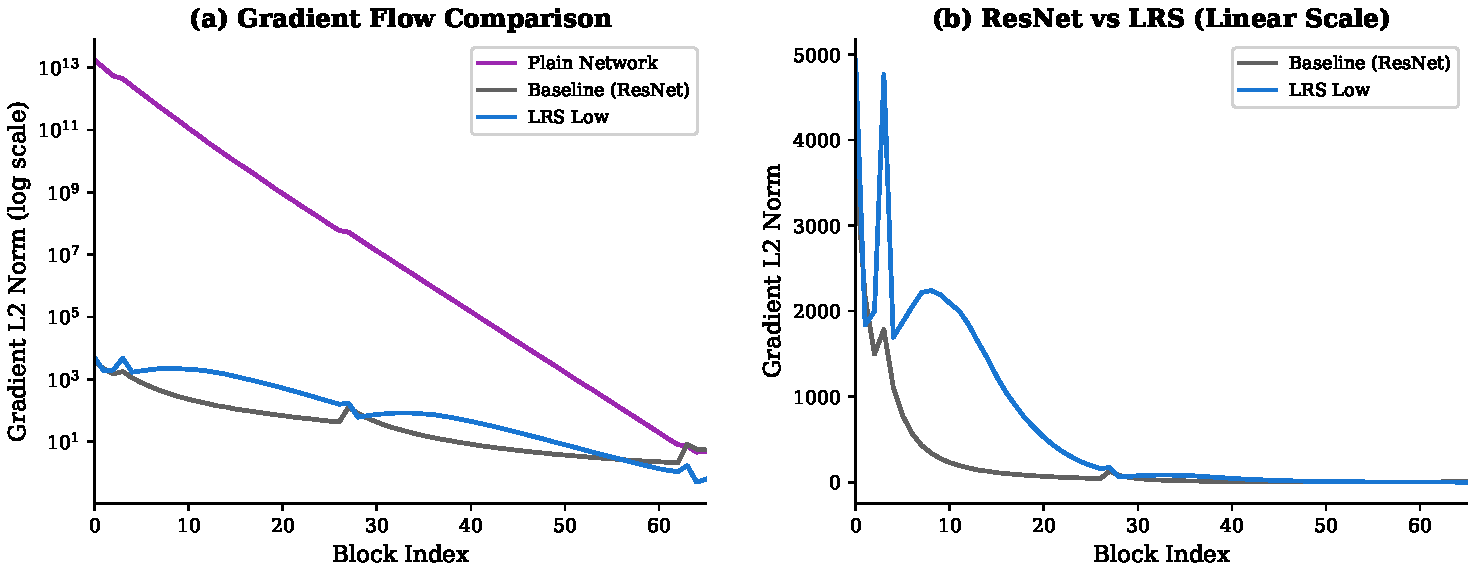
\includegraphics[width=\linewidth]{figures/fig0_gradient_flow.pdf}
    \caption{CIFAR-100에서 ResNet-200의 초기화 시점 블록별 기울기 L2 노름. (a) Skip connection이 없는 일반 네트워크는 초기 블록에서 기울기 폭발($>10^{13}$)을 보인다. Skip connection(ResNet)은 모든 블록에 걸쳐 기울기를 안정화한다. (b-c) LRS에서는 후반 블록이 거의 0에 가까운 기울기를 보이며, 이는 학습된 $\alpha \approx 0$을 반영한다---네트워크가 이 블록들을 학습하려 시도하지 않는다.}
    \label{fig:gradient_flow}
\end{figure}

본 연구에서는 분석 도구로서 \textbf{학습 가능한 잔차 스케일링(Learnable Residual Scaling, LRS)}을 제안한다. LRS는 블록당 단일 학습 가능 매개변수 $\alpha \in (0,1)$를 도입하여 $y = \alpha \cdot F(x) + (1-\alpha) \cdot x$로 정의한다. 두 계수의 합이 1이므로, 학습된 $\alpha$는 블록의 선호도를 직접 부호화한다: $\alpha \to 0$이면 블록은 효과적으로 항등(우회)이고, $\alpha \to 1$이면 완전한 변환을 수행한다. 학습 후 블록 전체의 $\alpha$ 값 분포는 네트워크의 \emph{유효 깊이}---입력을 실질적으로 변환하는 블록의 수---를 드러낸다.

LRS를 사용하여 네 가지 깊이(50, 101, 152, 200), 두 개의 CIFAR 데이터셋, 그리고 ImageNet에서 구성당 3개의 랜덤 시드로 체계적 실험을 수행했다. 본 연구의 기여는 다음과 같다:

\begin{enumerate}
    \item \textbf{깊이--$\alpha$ 스케일링 법칙}: 평균 수렴 $\alpha$는 네트워크 깊이에 따라 체계적으로 감소하며, 이 관계는 데이터셋에 크게 의존하지 않아 고유한 구조적 속성을 반영함을 시사한다.
    \item \textbf{유효 깊이는 명목 깊이보다 훨씬 작다}: 200층 네트워크(66개 블록)에서 5--6개 블록만이 $\alpha > 0.3$을 유지한다. 네트워크는 유효 깊이를 명목 깊이의 약 8\%로 자율적으로 압축한다.
    \item \textbf{초기화가 학습 가능성을 결정한다}: 잔차 선호 초기화 ($\alpha_0 \approx 0.88$)는 극단적 깊이에서 치명적 실패를 야기하는 반면, 항등 선호 초기화 ($\alpha_0 \approx 0.12$)는 모든 깊이에서 안정적이다.
\end{enumerate}

코드 및 모든 실험 결과는 \url{https://github.com/Wlsghdh/Learnable_Residual_Scaling}에서 확인할 수 있다.

%% ============================================================
\section{관련 연구}
\label{sec:related}

\subsection{잔차 네트워크와 Skip Connection}

ResNet~\cite{he2016deep}은 심층 네트워크에서의 기울기 소실을 완화하기 위해 skip connection을 도입했다. He et al.~\cite{he2016identity}은 identity mapping(사전 활성화 ResNet)이 기울기 흐름을 개선함을 추가로 보였다. Highway Network~\cite{srivastava2015highway}는 ResNet 이전에 게이트 기반 정보 흐름을 제안했지만, ResNet의 더 단순한 가산 숏컷이 실제로 더 효과적임이 입증되었다. Veit et al.~\cite{veit2016residual}은 ResNet을 다양한 길이의 경로들로 구성된 암묵적 앙상블로 재해석하여, 유효 경로가 명목 깊이보다 훨씬 짧다는 것을 보였다.

\subsection{잔차 스케일링 방법}

잔차 분기의 크기를 조정하는 연구가 여럿 수행되었다(Table~\ref{tab:comparison}).

\textbf{ReZero}~\cite{bachlechner2021rezero}는 잔차 분기에 스칼라 곱셈기 $\alpha = 0$을 초기화하여 ($y = x + \alpha F(x)$), 항등에서 시작함으로써 Transformer 학습을 안정화한다.

\textbf{SkipInit}~\cite{de2020batch}은 유사하게 잔차 분기에 학습 가능한 스칼라를 적용하며, batch normalization이 잔차 블록을 항등 쪽으로 편향시킨다는 것을 보였다.

\textbf{Fixup}~\cite{zhang2019fixup}은 잔차 분기의 마지막 층을 영으로 초기화하고 적절한 스케일링을 통해 정규화 없이 학습하는 방법을 제안했다.

\textbf{LayerScale}~\cite{touvron2021going}은 Vision Transformer에서 채널별 학습 가능 스케일링 벡터를 도입하여 심층 ViT의 학습을 안정화한다.

이 모든 방법은 $F(x)$만 조정하고 항등 연결 $x$는 가중치 1로 고정한다. 이와 대조적으로, LRS는 단일 매개변수를 통해 $F(x)$와 $x$ \textbf{양쪽의 상대적 가중치}를 학습하여, 각 블록의 기여도를 직접 측정할 수 있게 한다.

\begin{table}[t]
\centering
\caption{잔차 스케일링 방법의 비교. LRS만이 $F(x)$와 $x$ 간의 상대적 비율을 측정하므로, 유효 깊이의 분석 도구로 적합하다.}
\label{tab:comparison}
\begin{tabular}{lccc}
\toprule
\textbf{방법} & \textbf{수식} & \textbf{측정 가능} & \textbf{핵심 차이} \\
\midrule
ReZero & $y = x + \alpha F(x)$ & $|F(x)|$ 스케일 & $x$ 가중치 1로 고정 \\
SkipInit & $y = x + \alpha F(x)$ & $|F(x)|$ 스케일 & $x$ 가중치 1로 고정 \\
LayerScale & $y = x + \Lambda F(x)$ & 채널별 $|F(x)|$ & $x$ 가중치 1로 고정 \\
Fixup & $y = x + \alpha F(x)$ & $|F(x)|$ 스케일 & 마지막 층 영 초기화 \\
\textbf{LRS (본 연구)} & $\mathbf{y = \alpha F(x) + (1{-}\alpha)x}$ & $\mathbf{F(x):x}$ \textbf{비율} & \textbf{양쪽 모두 조정} \\
\bottomrule
\end{tabular}
\end{table}

\subsection{유효 깊이와 네트워크 중복성}

유효 깊이의 개념은 다양한 관점에서 탐구되어 왔다. Huang et al.~\cite{huang2016deep}은 학습 중 잔차 블록을 무작위로 제거하는 확률적 깊이(stochastic depth)를 제안하여 모든 블록이 필요하지는 않음을 보였다. 더 최근에는 복권 가설(lottery ticket hypothesis)~\cite{frankle2019lottery}이 대규모 네트워크가 전체 네트워크의 성능에 필적하는 작은 하위 네트워크를 포함하고 있음을 보였다. 본 연구는 보완적인 관점을 제공한다: 블록을 가지치기하거나 제거하는 대신, 학습된 $\alpha$ 값을 통해 네트워크 \emph{스스로}가 어떤 블록을 필수적으로 간주하는지 드러내게 한다.

%% ============================================================
\section{방법}
\label{sec:method}

\subsection{학습 가능한 잔차 스케일링}

표준 잔차 블록 출력 $y = F(x) + x$를 다음과 같이 재정의한다:
\begin{equation}
    y = \alpha \cdot F(x) + (1 - \alpha) \cdot x
    \label{eq:lrs}
\end{equation}
여기서 $\alpha = \sigma(\theta)$이고, $\theta$는 블록당 학습 가능한 스칼라 매개변수이며, $\sigma$는 $\alpha \in (0, 1)$로 제약하는 sigmoid 함수이다.

\textbf{설계 근거.} Sigmoid 매개변수화는 두 가지 목적을 갖는다. 첫째, $\alpha + (1 - \alpha) = 1$이므로, $F(x)$와 $x$ 간의 \textbf{상대적 비율}이 직접 해석 가능하다: $\alpha = 0.14$는 블록이 변환에 14\%, 항등에 86\%의 가중치를 할당함을 의미한다. 둘째, 유계 범위가 수치적 안정성을 보장한다.

$\alpha$의 의미는 유효 깊이의 자연스러운 정의를 제공한다:
\begin{itemize}
    \item $\alpha \to 0$: 블록이 효과적으로 우회됨 ($y \approx x$); 네트워크의 유효 깊이에 기여하지 않는다.
    \item $\alpha = 0.5$: 동등한 비율, 표준 ResNet 블록과 동일하다.
    \item $\alpha \to 1$: 블록이 완전한 변환을 수행함 ($y \approx F(x)$).
\end{itemize}

$\alpha$가 작은 블록은 네트워크가 크게 건너뛰기로 선택한 블록이다. 네트워크의 \textbf{유효 깊이}는 의미 있는 임계값 이상의 $\alpha$를 가진 블록의 수이다.

\begin{figure}[t]
    \centering
    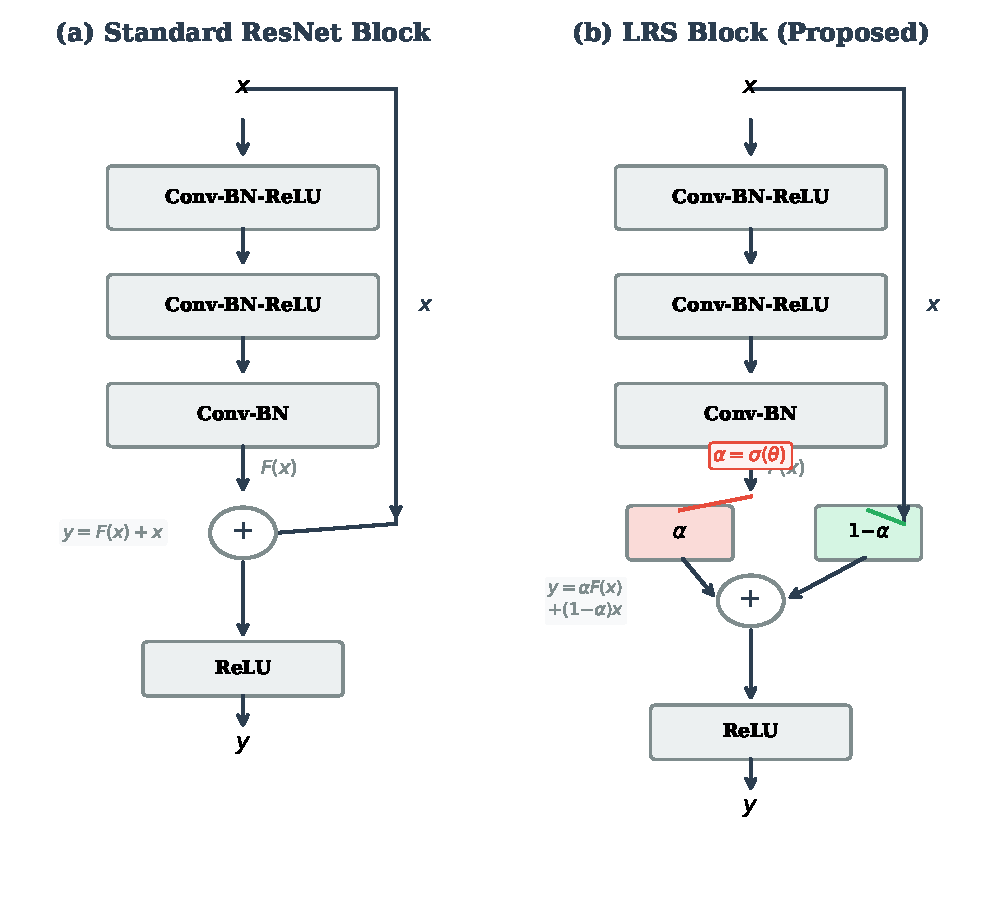
\includegraphics[width=0.85\linewidth]{figures/fig1_block_diagram.pdf}
    \caption{LRS 블록의 계산 그래프. 학습 가능한 매개변수 $\alpha = \sigma(\theta) \in (0,1)$가 잔차 변환 $F(x)$와 항등 숏컷 $x$의 상대적 기여도를 제어한다. 학습 후, $\alpha$는 블록이 입력을 능동적으로 변환하는지 효과적으로 항등 우회로 작동하는지를 드러낸다.}
    \label{fig:lrs_block}
\end{figure}

\subsection{기울기 흐름 분석}

LRS 블록을 통한 역전파는 다음과 같다:
\begin{equation}
    \frac{\partial \mathcal{L}}{\partial x} = \frac{\partial \mathcal{L}}{\partial y} \left[ (1 - \alpha) + \alpha \cdot F'(x) \right]
    \label{eq:grad}
\end{equation}

$L$개 블록을 통한 전체 기울기:
\begin{equation}
    \frac{\partial \mathcal{L}}{\partial x_0} = \frac{\partial \mathcal{L}}{\partial y_L} \cdot \prod_{i=1}^{L} \left[ (1 - \alpha_i) + \alpha_i \cdot F'_i(x_i) \right]
    \label{eq:total_grad}
\end{equation}

이 곱 구조는 깊이--$\alpha$ 관계를 설명한다. 곱이 $L$개 블록에 걸쳐 안정적으로 유지되려면, 각 인수 $(1 - \alpha_i) + \alpha_i F'_i$가 1에 가까워야 한다. $\alpha_i$가 작으면 인수가 $F'_i$에 관계없이 $(1 - \alpha_i) \approx 1$에 접근하여 기울기 안정성을 보장한다. $L$이 증가하면 곱을 1 근처로 유지하기 위해 더 작은 $\alpha_i$ 값이 필요하다. 이것이 더 깊은 네트워크가 더 작은 $\alpha$ 값으로 수렴해야 하는 이론적 근거를 제공한다.

반대로, $\alpha_i$가 크면 (1에 가까우면) 인수가 $\approx F'_i$가 되어, 기울기 곱이 기울기 소실에 취약한 일반(비잔차) 네트워크의 것으로 퇴화한다. 이것이 잔차 선호 초기화 ($\alpha_0 \approx 0.88$)가 극단적 깊이에서 학습 붕괴를 야기하는 이유를 설명한다.

\subsection{초기화 변형}

수렴과 민감도를 연구하기 위해 세 가지 초기화 전략으로 실험한다(Table~\ref{tab:init_variants}):

\begin{table}[t]
\centering
\caption{$\alpha$ 초기화에 따른 LRS 모델 변형. 세 가지 모두 다른 시작점에서 출발하여 $\alpha$가 동일한 최적값으로 수렴하는지 검증한다.}
\label{tab:init_variants}
\begin{tabular}{lccc}
\toprule
\textbf{변형} & $\theta_0$ & $\alpha_0$ & \textbf{초기 편향} \\
\midrule
LRS Low  & $-2.0$ & $\approx 0.12$ & 항등 선호 \\
LRS Mid  & $0.0$  & $0.50$         & 균형 (표준 ResNet) \\
LRS High & $+2.0$  & $\approx 0.88$ & 잔차 선호 \\
\bottomrule
\end{tabular}
\end{table}

이 세 가지 초기화는 탐침 역할을 한다: 최적화 지형에 단일 분지가 있다면 세 가지 모두 동일한 $\alpha$로 수렴해야 하고, 초기화가 중요하다면 발산이 예상되어 유효 깊이 결정에서 초기 조건의 역할을 드러낸다.

%% ============================================================
\section{실험}
\label{sec:experiments}

\subsection{실험 설정}
\label{sec:setup}

\textbf{데이터셋.} 체계적 분석을 위한 CIFAR-10 (10 클래스, 50K/10K 학습/테스트)과 CIFAR-100 (100 클래스, 50K/10K); 대규모 검증을 위한 ImageNet (1000 클래스, 1.28M/50K).

\textbf{아키텍처.} CIFAR 실험에는 Bottleneck ResNet-50/101/152/200; ImageNet에는 ResNet-50. 깊이별 잔차 블록 수: 50->16, 101->33, 152->50, 200->66.

\textbf{학습 (CIFAR).} 모멘텀 0.9, 가중치 감쇠 $10^{-4}$의 SGD; 초기 학습률 0.1, 코사인 어닐링; 5 에포크 선형 워밍업; 총 100 에포크; 배치 크기 128.

\textbf{학습 (ImageNet).} 모멘텀 0.9, 가중치 감쇠 $10^{-4}$의 SGD; 초기 학습률 0.1, 코사인 어닐링; 5 에포크 워밍업; 100 에포크; 배치 크기 256.

\textbf{시드 및 보고.} 모든 CIFAR 실험은 3개의 랜덤 시드(42, 123, 456)를 사용한다. 평균 +/- 표준편차를 보고한다. ImageNet 실험은 계산 비용으로 인해 단일 시드를 사용한다.

\textbf{모델.} 다섯 가지 주요 모델을 평가한다: Baseline (표준 ResNet), LRS Low ($\alpha_0 \approx 0.12$), LRS Mid ($\alpha_0 = 0.50$), LRS High ($\alpha_0 \approx 0.88$), ReZero ($\alpha_0 = 0$, $y = x + \alpha F(x)$). 기존 방법과의 비교를 위해 SkipInit, Fixup, LayerScale도 추가로 평가한다.

\subsection{깊이에 따른 Alpha 수렴}
\label{sec:alpha_convergence}

먼저 핵심 질문을 검토한다: 네트워크가 선호하는 $\alpha$는 깊이에 따라 어떻게 변하는가? Table~\ref{tab:depth_alpha}는 3개 시드 평균으로 CIFAR-100에서 세 가지 LRS 초기화 변형 모두의 평균 수렴 $\alpha$ 값을 제시한다.

\begin{table}[t]
\centering
\caption{CIFAR-100에서의 깊이별 평균 수렴 $\alpha$ 값 (3-시드 평균). 매우 다른 초기값 ($\alpha_0 = 0.12, 0.50, 0.88$)에서 시작함에도, Low와 Mid 변형은 각 깊이에서 유사한 최종 값으로 수렴하는 반면, High는 더 깊은 깊이에서 발산한다.}
\label{tab:depth_alpha}
\begin{tabular}{lcccc}
\toprule
\textbf{깊이} & \textbf{블록 수} & \textbf{LRS Low} & \textbf{LRS Mid} & \textbf{LRS High} \\
\midrule
50  & 16 & 0.34 & 0.35 & 0.36 \\
101 & 33 & 0.18 & 0.20 & 0.21 \\
152 & 50 & 0.13 & 0.15 & 0.23 \\
200 & 66 & 0.11 & 0.13 & 0.28 \\
\bottomrule
\end{tabular}
\end{table}

몇 가지 중요한 관찰이 도출된다:

\textbf{깊이에 따른 체계적 감소.} 수렴된 $\alpha$는 모든 초기화 변형에서 깊이에 따라 단조롭게 감소한다. LRS Low의 경우 $\alpha$는 0.34 (깊이 50)에서 0.11 (깊이 200)로 감소하며, 이는 가장 깊은 구성에서 네트워크가 블록 변환에 11\%의 가중치만 할당함을 나타낸다. 즉, 블록이 추가될수록 각 블록의 기여가 줄어든다.

\textbf{초기화 간 부분적 수렴.} 깊이 50에서 세 변형 모두 거의 동일한 값(0.34--0.36)으로 수렴하여 잘 정의된 최적점이 있음을 나타낸다. 그러나 깊이 200에서는 수렴이 깨진다: LRS High는 0.28에 정착하여 Low와 Mid의 0.11--0.13 범위보다 상당히 높다. 이 발산은 심각한 성능 저하(Section~\ref{sec:init_sensitivity})와 결합되어, LRS High가 극단적 깊이에서 차선의 분지에 갇힘을 나타낸다.

\textbf{데이터 독립성.} 수렴된 $\alpha$ 값은 CIFAR-10과 CIFAR-100 간에 매우 유사하여(간결성을 위해 별도로 표시하지 않음), 깊이--$\alpha$ 관계가 과제 복잡성이 아닌 구조적 속성에 의해 지배됨을 시사한다.

\begin{figure}[t]
    \centering
    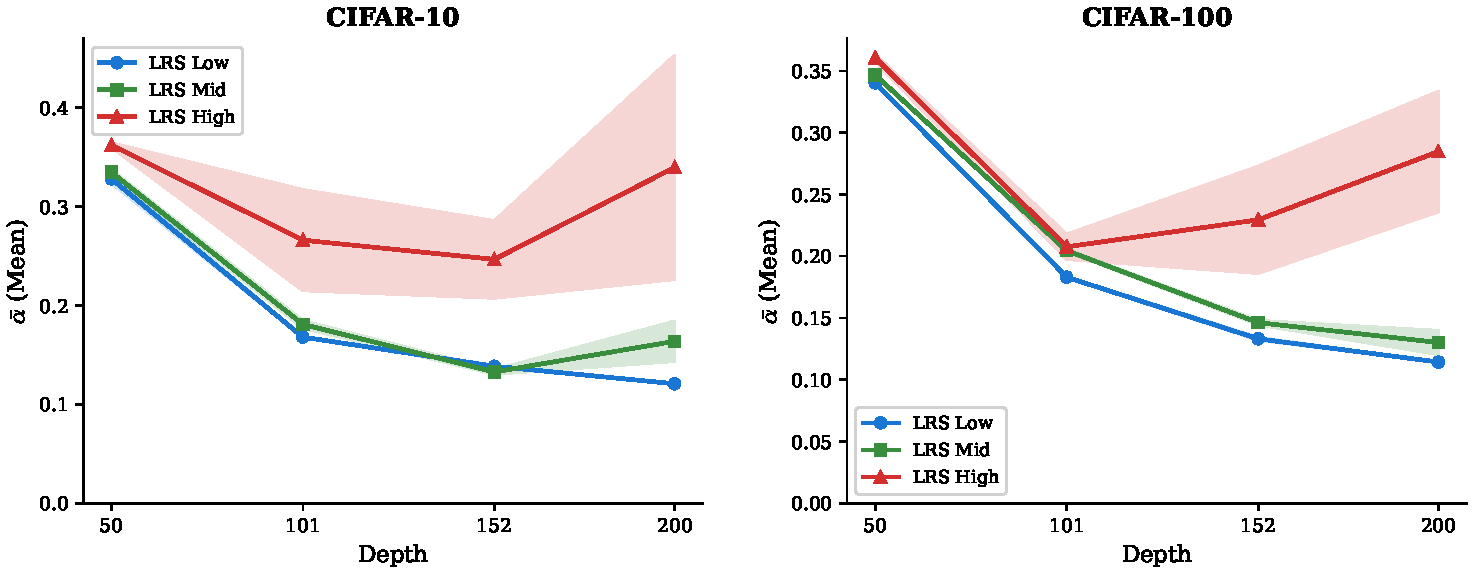
\includegraphics[width=0.85\linewidth]{figures/fig2_alpha_depth.pdf}
    \caption{CIFAR-100에서 세 가지 초기화 변형에 대한 네트워크 깊이의 함수로서의 평균 수렴 $\alpha$. 얕은 깊이에서는 모든 초기화가 유사한 값으로 수렴하지만, 극단적 깊이에서는 High 초기화가 최적화 어려움으로 인해 발산한다.}
    \label{fig:alpha_convergence}
\end{figure}

\subsection{학습 중 Alpha 궤적}
\label{sec:alpha_trajectory}

Figure~\ref{fig:alpha_trajectory}는 학습 과정에서 평균 $\alpha$가 어떻게 변화하는지 보여준다. 세 가지 초기화 모두 빠른 초기 조정을 보인다: LRS Low는 0.12에서 약간 증가하고, LRS Mid는 0.50에서 감소하며, LRS High는 0.88에서 감소한다(학습이 성공할 때). 궤적은 대체로 처음 20--30 에포크 내에 안정화되며, 미세 조정은 학습 종료까지 계속된다.

깊이 200에서 LRS High의 궤적은 실패 모드를 드러낸다: $\alpha$가 느리게 감소하지만 Low와 Mid가 달성한 값에 도달하지 못하고 약 0.28에 머물러 있다. 네트워크는 높은 $\alpha$ 값으로 인한 초기 기울기 저하에서 회복할 수 없다.

\begin{figure}[t]
    \centering
    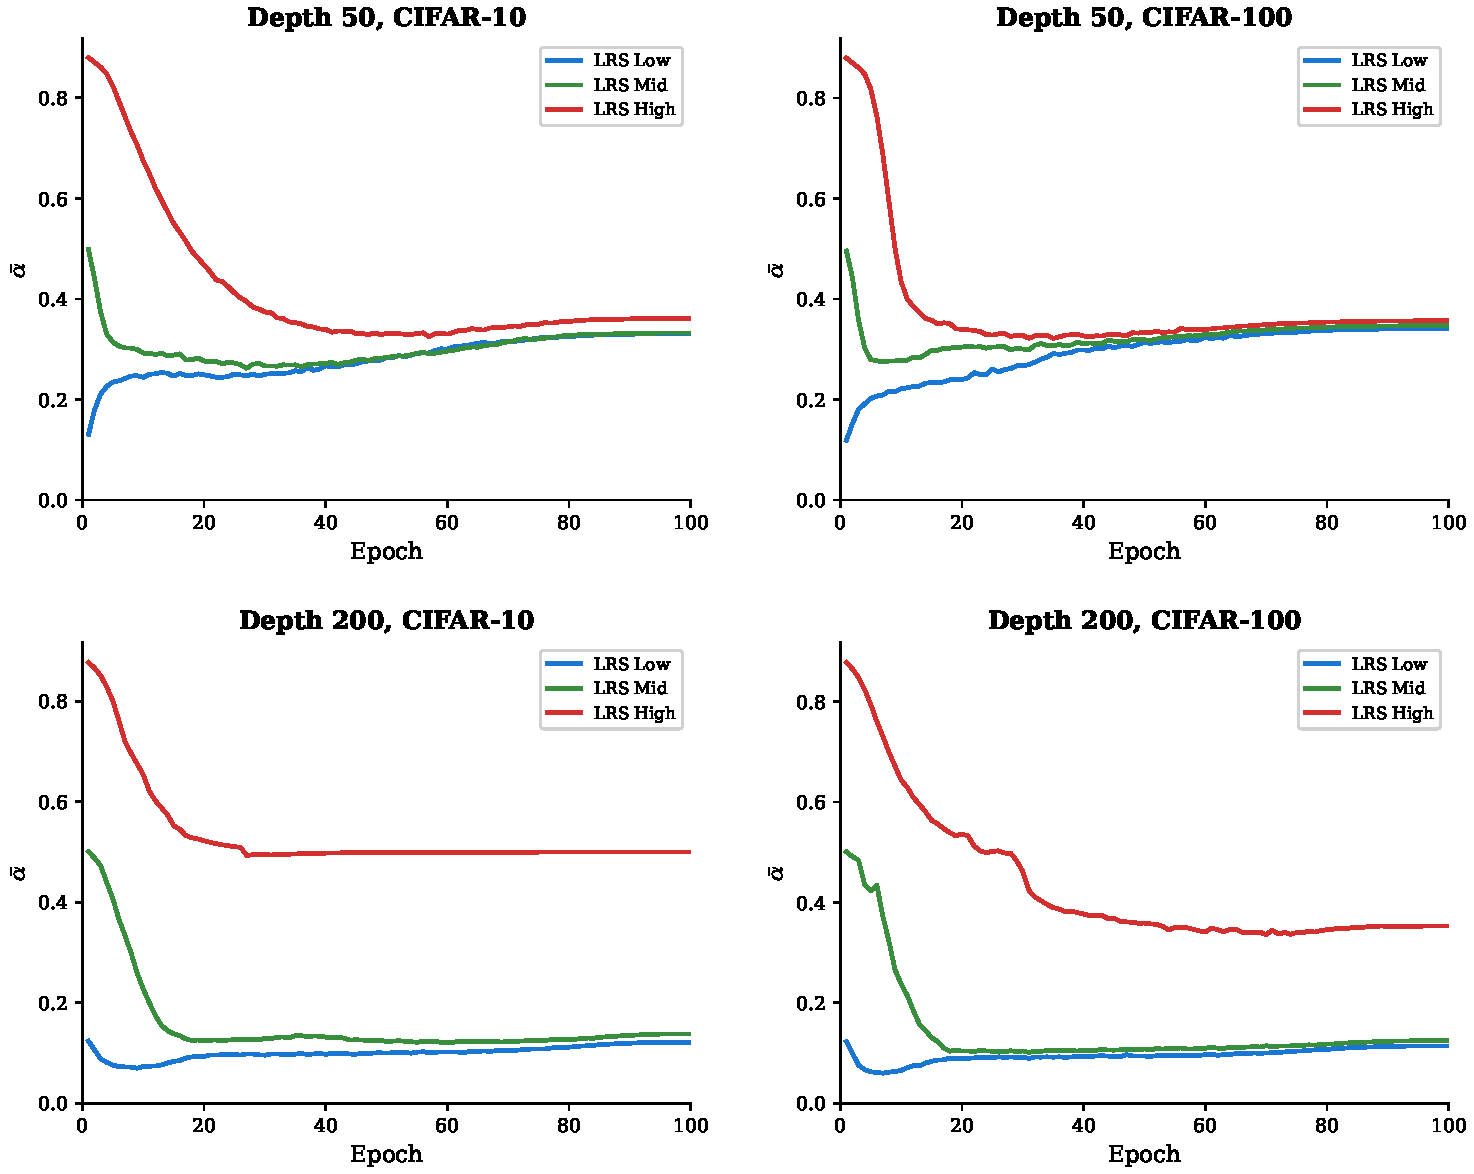
\includegraphics[width=\linewidth]{figures/fig3_alpha_trajectory.pdf}
    \caption{에포크에 따른 평균 $\alpha$ 궤적. 왼쪽: 중간 깊이에서 다른 시작점으로부터의 성공적 수렴. 오른쪽: 깊이 200에서 LRS High가 최적 범위로 수렴하지 못하고 차선의 $\alpha \approx 0.28$에 갇힌다.}
    \label{fig:alpha_trajectory}
\end{figure}

\subsection{블록별 Alpha 분포}
\label{sec:perblock}

모든 블록에 대한 평균 $\alpha$ 값은 중요한 구조를 숨긴다. Figure~\ref{fig:perblock_alpha}는 200층 네트워크(66개 블록, LRS Low, CIFAR-100)의 블록별 $\alpha$ 분포를 보여준다.

분포는 눈에 띄는 패턴을 드러낸다:

\textbf{다운샘플링 블록은 높은 $\alpha$를 가진다.} 각 스테이지의 첫 번째 블록(공간 다운샘플링이 발생하고 채널 차원이 변경되는 곳)은 0.42에서 0.96 사이의 $\alpha$ 값을 유지하며, 이는 평균의 약 5배이다. 이 블록들은 우회할 수 없는 필수적인 특징 변환을 수행한다.

\textbf{일반 블록은 낮은 $\alpha$를 가진다.} 각 스테이지 내에서 다운샘플링이 아닌 블록들은 0.06--0.15의 $\alpha$ 값을 가지며, 이 값은 스테이지 끝 쪽으로 갈수록 감소하는 경향이 있다. 이 블록들 대부분은 거의 항등 연산이다.

\textbf{스테이지 내 $\alpha$ 감소.} 주어진 스테이지 내에서 다운샘플링 지점으로부터 멀어질수록 블록의 $\alpha$ 값이 점진적으로 작아지는 경향이 있어, 한계 기여의 체감을 시사한다.

\begin{figure}[t]
    \centering
    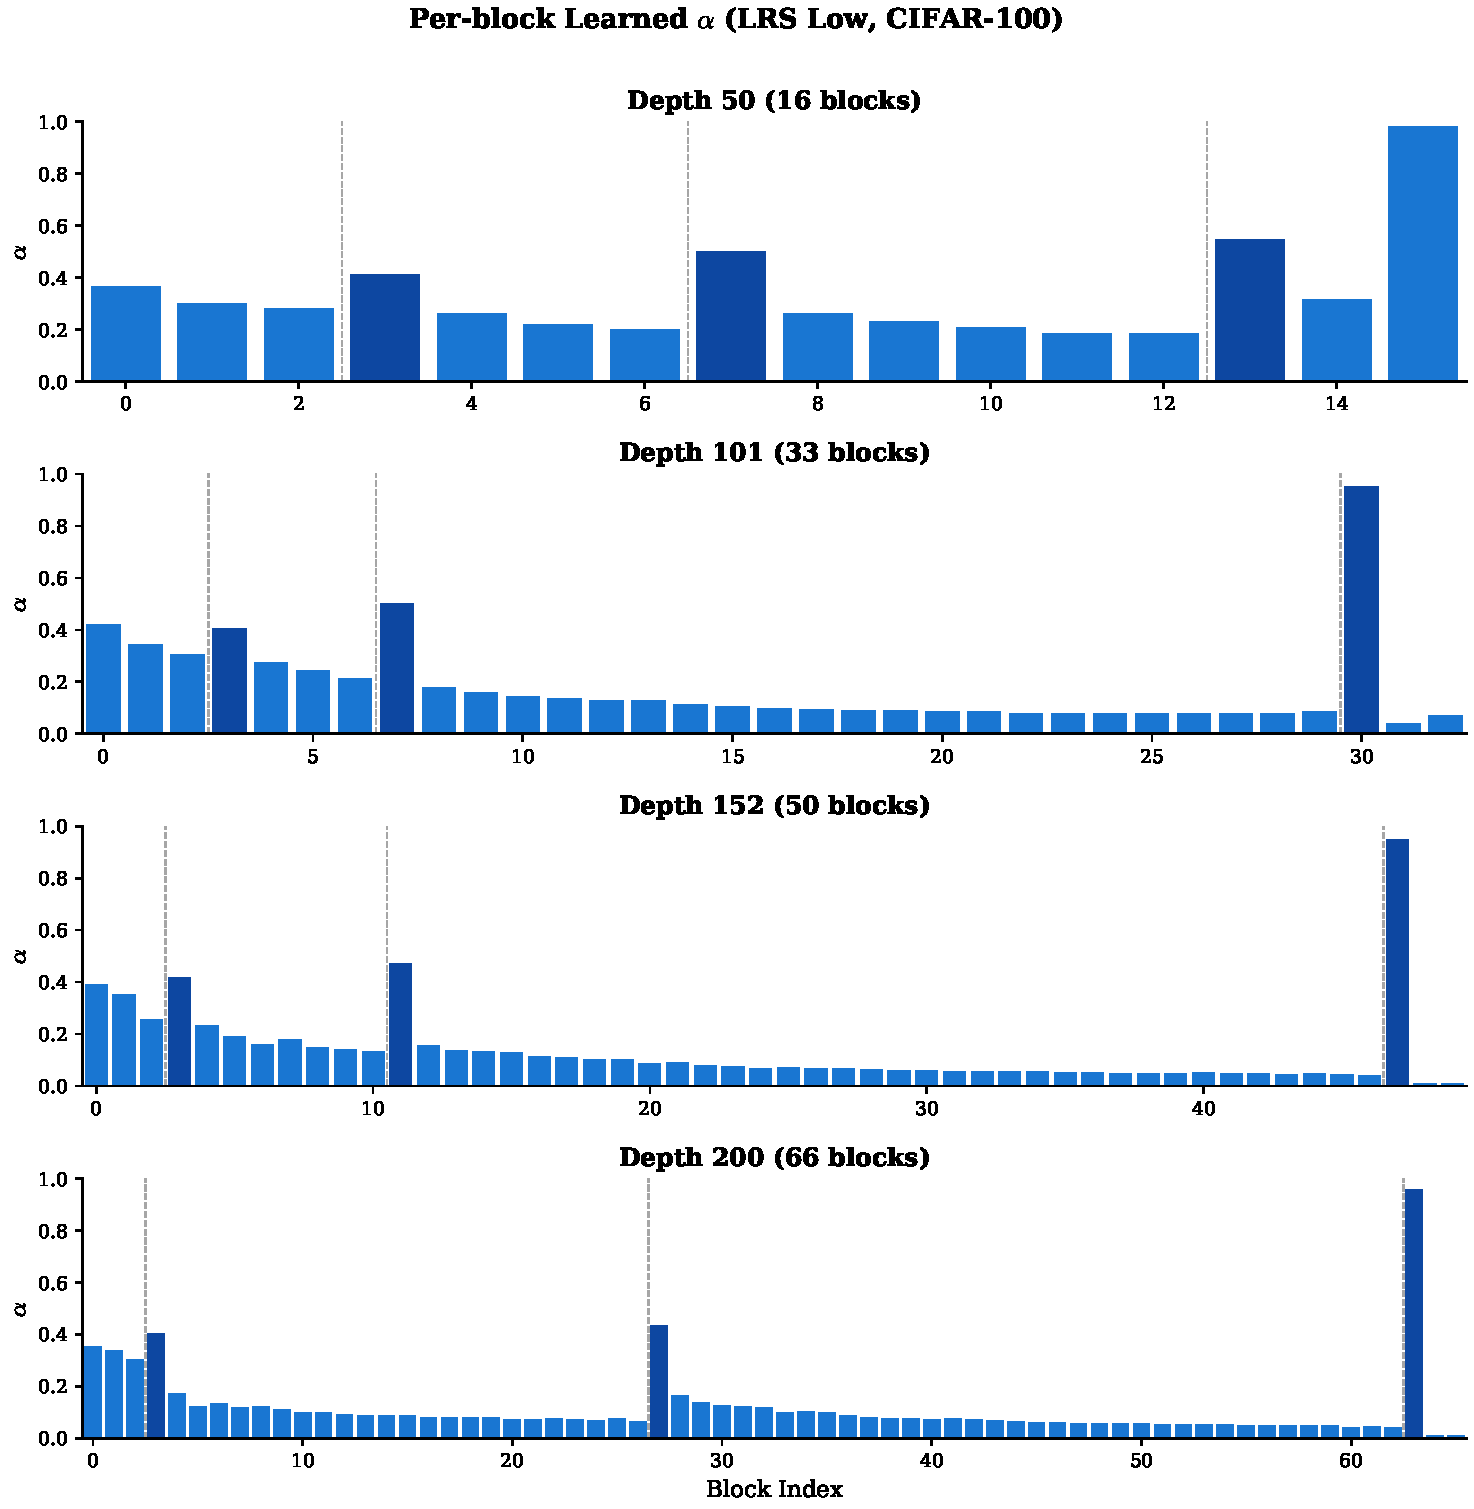
\includegraphics[width=\linewidth]{figures/fig4_perblock_alpha.pdf}
    \caption{200층 ResNet (66개 블록, LRS Low, CIFAR-100)의 블록별 $\alpha$ 값. 스테이지 경계(다운샘플링 블록)는 점선으로 표시된다. 다운샘플링 블록은 높은 $\alpha$를 유지하는 반면, 스테이지 내 대부분의 블록은 거의 0에 가까운 값으로 수렴한다.}
    \label{fig:perblock_alpha}
\end{figure}

\begin{figure}[t]
    \centering
    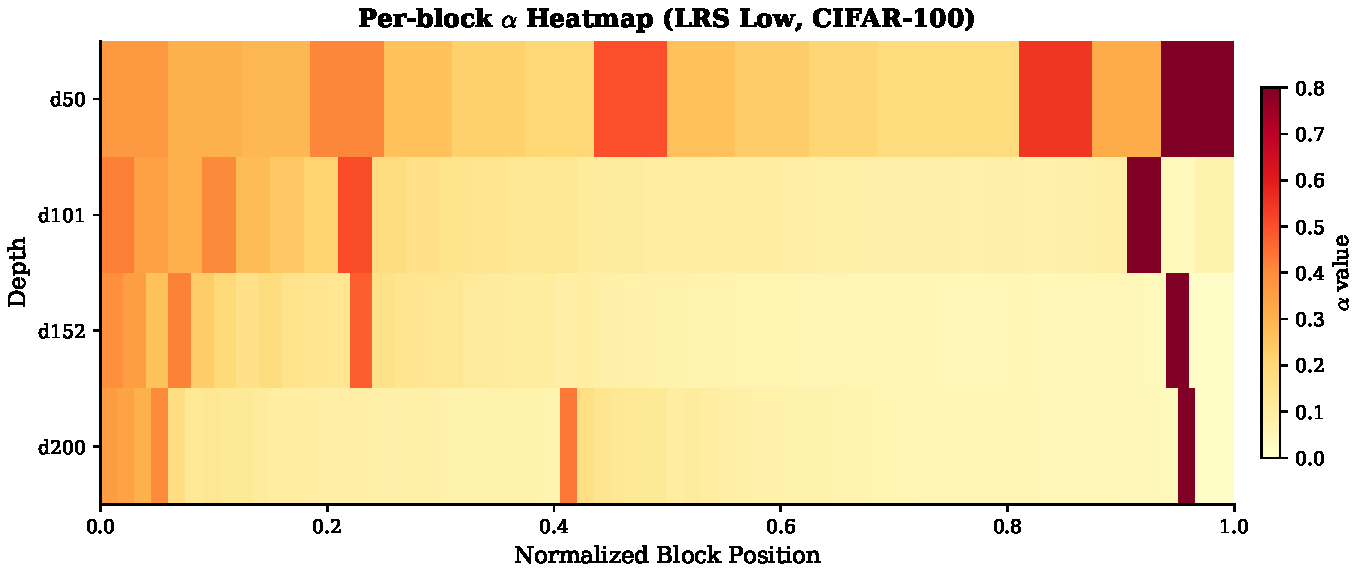
\includegraphics[width=0.85\linewidth]{figures/fig8_heatmap.pdf}
    \caption{스테이지별로 그룹화된 블록별 $\alpha$ 분포의 상세 뷰. 스테이지 경계에서 높은 $\alpha$ 이후 각 스테이지 내에서의 감쇠라는 일관된 패턴이 네 스테이지 모두에서 명확하게 나타난다.}
    \label{fig:perblock_detail}
\end{figure}

\subsection{유효 깊이 분석}
\label{sec:effective_depth}

블록별 $\alpha$ 분포는 \emph{유효 깊이}---입력을 의미 있게 변환하는 블록의 수---를 직접 측정할 수 있게 한다. $\alpha > 0.3$을 임계값으로 사용하면(30\% 이상의 변환을 기여하는 블록), 다음과 같은 결과를 얻는다:

\begin{table}[t]
\centering
\caption{CIFAR-100에서 ResNet-200 (66개 블록)의 유효 깊이 분석, LRS Low. 네트워크는 명목 깊이의 극히 일부만 사용한다.}
\label{tab:effective_depth}
\begin{tabular}{lcc}
\toprule
\textbf{지표} & \textbf{값} & \textbf{해석} \\
\midrule
명목 블록 수 & 66 & 전체 잔차 블록 \\
$\alpha > 0.3$인 블록 & 5--6 & 능동적으로 변환 중 \\
유효 깊이 비율 & ~8\% & 사용된 블록 비율 \\
평균 $\alpha$ (일반 블록) & 0.06--0.15 & 거의 항등 \\
평균 $\alpha$ (다운샘플링 블록) & 0.42--0.96 & 능동적 변환 \\
\bottomrule
\end{tabular}
\end{table}

이 발견은 놀라운 함의를 가진다: \textbf{200층 ResNet은 약 5--6개 블록의 유효 깊이를 자율적으로 선택한다}. 나머지 60개 이상의 블록은 주로 항등 숏컷으로 작동하여, 최소한의 변환으로 정보를 전달한다. 네트워크는 깊을 수 있는 용량이 주어졌음에도 불구하고 사실상 얕아지기를 선택한 것이다.

이는 ResNet에서 유효 경로가 전체 네트워크 깊이보다 훨씬 짧다는 것을 보인 Veit et al.~\cite{veit2016residual}의 앙상블 해석과 일치한다. LRS는 이 현상에 대한 직접적인 블록별 측정을 제공한다.

\textbf{임계값 민감도.} ``활성'' 블록의 기준으로 $\alpha > 0.3$을 사용한 것은 다소 자의적일 수 있다. 이 문제를 해결하기 위해 두 가지 보완 분석을 제시한다.

첫째, Table~\ref{tab:threshold_sensitivity}는 다양한 임계값에서의 유효 깊이를 보여준다. 어떤 임계값을 선택하더라도 두 가지 패턴은 변하지 않는다: (1) 유효 깊이 비율은 명목 깊이가 증가함에 따라 단조 감소하며, (2) 얕은 네트워크와 깊은 네트워크 사이의 차이는 모든 임계값에서 현저하다.

\begin{table}[t]
\centering
\caption{LRS Low의 CIFAR-100에서 임계값별 유효 깊이 비율 (3-seed 평균). 명목 깊이가 증가할수록 유효 깊이가 감소하는 패턴은 모든 임계값에서 일관적이다.}
\label{tab:threshold_sensitivity}
\begin{tabular}{lcccc}
\toprule
\textbf{임계값} & \textbf{Depth 50} & \textbf{Depth 101} & \textbf{Depth 152} & \textbf{Depth 200} \\
\midrule
$\alpha > 0.10$ & 100\% & 54\% & 40\% & 28\% \\
$\alpha > 0.20$ & 83\% & 27\% & 15\% & 10\% \\
$\alpha > 0.30$ & 40\% & 18\% & 11\% & 7\% \\
$\alpha > 0.40$ & 25\% & 12\% & 7\% & 5\% \\
\bottomrule
\end{tabular}
\end{table}

둘째, 임계값이 필요 없는 지표를 정의한다: $D_\text{eff} = \sum_{i=1}^{N} \alpha_i$. 이는 모든 블록의 기여도 합으로 유효 깊이를 나타낸다.

\begin{table}[t]
\centering
\caption{임계값 없는 유효 깊이 ($D_\text{eff} = \sum \alpha_i$), LRS Low, CIFAR-100. 블록 수가 depth 50에서 200으로 4배 증가하지만, $D_\text{eff}$는 1.4배만 증가한다.}
\label{tab:deff}
\begin{tabular}{lccc}
\toprule
\textbf{Depth} & \textbf{블록 수 ($N$)} & $\mathbf{D_\text{eff} = \sum \alpha_i}$ & $\mathbf{D_\text{eff}/N}$ \\
\midrule
50  & 16 & 5.4 & 34.0\% \\
101 & 33 & 6.0 & 18.3\% \\
152 & 50 & 6.7 & 13.3\% \\
200 & 66 & 7.5 & 11.4\% \\
\bottomrule
\end{tabular}
\end{table}

$D_\text{eff}$ 지표는 임계값 없이도 핵심 발견을 확인해준다: 블록 수를 4배 늘려도 (16 $\to$ 66) 유효 깊이는 40\%만 증가한다 (5.4 $\to$ 7.5). 네트워크는 블록을 추가하지만 거의 사용하지 않는다.

\begin{figure}[t]
    \centering
    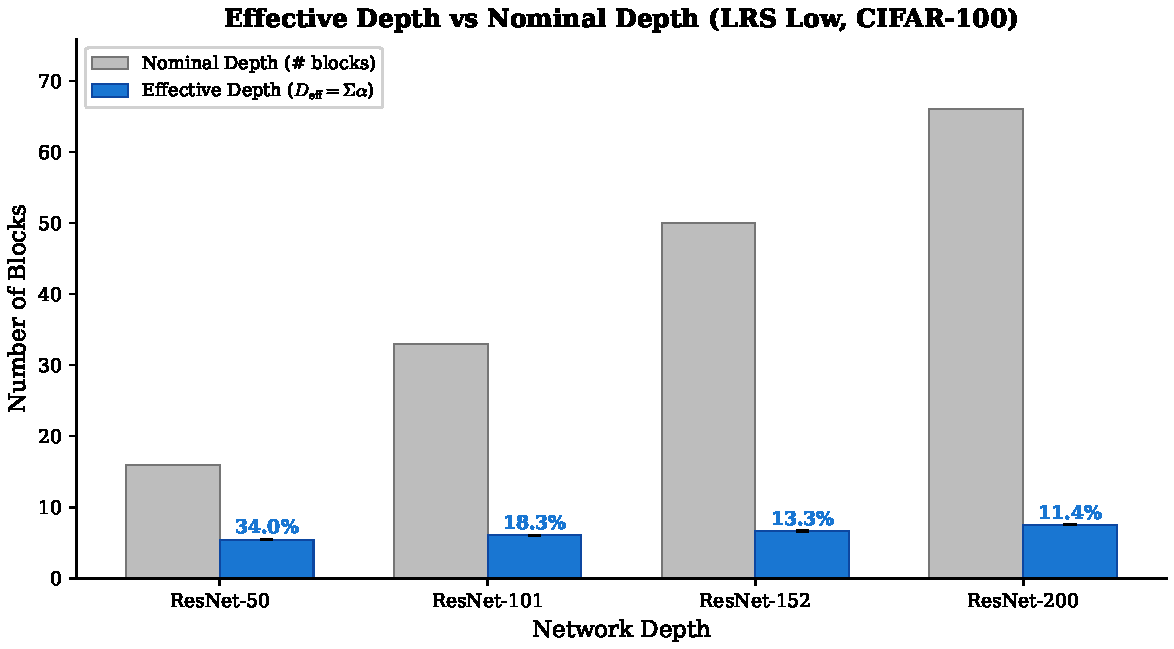
\includegraphics[width=0.85\linewidth]{figures/fig5_effective_depth.pdf}
    \caption{유효 깊이 시각화. 각 블록은 $\alpha$ 값에 따라 색칠된다: 어두운 블록 ($\alpha > 0.3$)은 입력을 능동적으로 변환하고, 밝은 블록 ($\alpha < 0.15$)은 거의 항등 우회이다. ResNet-200의 66개 블록 중 5--6개만이 ``어두운'' 블록이며, 이는 네트워크의 유효 깊이가 명목 깊이의 약 8\%임을 보여준다.}
    \label{fig:effective_depth}
\end{figure}

\subsection{초기화 민감도와 LRS High 실패}
\label{sec:init_sensitivity}

세 가지 LRS 초기화는 깊이가 증가함에 따라 학습 안정성에서 극적인 차이를 드러낸다. Table~\ref{tab:cifar10}과 Table~\ref{tab:cifar100}에 전체 정확도 결과를 제시한다.

\begin{table}[t]
\centering
\caption{CIFAR-10에서의 테스트 정확도 (\%) (3-시드 평균 $\pm$ 표준편차). LRS High는 점진적 저하와 깊이 200에서의 치명적 실패를 보인다.}
\label{tab:cifar10}
\begin{tabular}{lccccc}
\toprule
\textbf{깊이} & \textbf{Baseline} & \textbf{LRS Low} & \textbf{LRS Mid} & \textbf{LRS High} & \textbf{ReZero} \\
\midrule
50  & 94.53$\pm$0.14 & \textbf{94.83$\pm$0.13} & 94.77$\pm$0.03 & 94.27$\pm$0.17 & 94.60$\pm$0.28 \\
101 & 95.37$\pm$0.11 & \textbf{95.44$\pm$0.12} & 95.15$\pm$0.11 & 94.28$\pm$0.29 & 95.38$\pm$0.21 \\
152 & 95.95$\pm$0.06 & 95.73$\pm$0.10 & 95.60$\pm$0.15 & 93.78$\pm$0.87 & \textbf{95.99$\pm$0.06} \\
200 & 95.98$\pm$0.15 & \textbf{96.10$\pm$0.12} & 94.36$\pm$0.92 & 67.25$\pm$43.65 & 96.02$\pm$0.16 \\
\bottomrule
\end{tabular}
\end{table}

\begin{table}[t]
\centering
\caption{CIFAR-100에서의 테스트 정확도 (\%) (3-시드 평균 $\pm$ 표준편차). LRS High의 점진적 실패는 더 어려운 과제에서 더욱 두드러진다.}
\label{tab:cifar100}
\begin{tabular}{lccccc}
\toprule
\textbf{깊이} & \textbf{Baseline} & \textbf{LRS Low} & \textbf{LRS Mid} & \textbf{LRS High} & \textbf{ReZero} \\
\midrule
50  & 77.18$\pm$0.36 & 77.02$\pm$0.20 & 76.72$\pm$0.40 & 75.22$\pm$0.45 & 76.12$\pm$0.09 \\
101 & \textbf{79.29$\pm$0.23} & 78.85$\pm$0.14 & 78.34$\pm$0.19 & 75.16$\pm$1.69 & 78.04$\pm$0.48 \\
152 & \textbf{80.42$\pm$0.22} & 80.28$\pm$0.38 & 78.57$\pm$0.60 & 71.66$\pm$3.40 & 79.72$\pm$0.10 \\
200 & \textbf{80.72$\pm$0.17} & 80.65$\pm$0.01 & 76.07$\pm$1.59 & 37.50$\pm$29.20 & 80.14$\pm$0.17 \\
\bottomrule
\end{tabular}
\end{table}

결과는 초기화 안전성의 명확한 계층 구조를 드러낸다:

\textbf{LRS Low ($\alpha_0 \approx 0.12$)}는 모든 깊이에서 baseline과 동등하거나 약간 높은 성능을 보이며, 시드 간 분산이 낮다. 깊이 200에서 CIFAR-10 최고 결과(96.10\%)를 달성하고 CIFAR-100에서도 거의 최고(80.65\%)를 달성한다.

\textbf{LRS Mid ($\alpha_0 = 0.50$)}는 중간 깊이에서 안정적이지만 깊이 200에서 저하된다(CIFAR-100: 76.07+/-1.59\%), 증가하는 분산이 최적화 불안정성을 신호한다.

\textbf{LRS High ($\alpha_0 \approx 0.88$)}는 깊이에 따른 점진적 저하를 보이며, 깊이 200에서 치명적 실패에 이른다: CIFAR-10에서 67.25+/-43.65\%, CIFAR-100에서 37.50+/-29.20\%. 매우 큰 표준편차는 일부 시드가 완전히 실패하고 다른 시드는 부분적으로 회복됨을 나타낸다.

실패 메커니즘은 기울기 분석(Equation~\ref{eq:total_grad})에서 명확하다: $\alpha_0 = 0.88$에서 각 기울기 인수의 항등 성분은 $1 - 0.88 = 0.12$에 불과하다. 66개 블록을 통해 기울기 보존 기준선은 $0.12^{66}$이며, 이는 천문학적으로 작아 빠른 $\alpha$ 조정 없이는 학습이 불가능하다. 그러나 빠른 $\alpha$ 조정 자체에 기울기가 필요하여---닭과 달걀 문제를 만들어 학습 붕괴를 야기한다.

\begin{figure}[t]
    \centering
    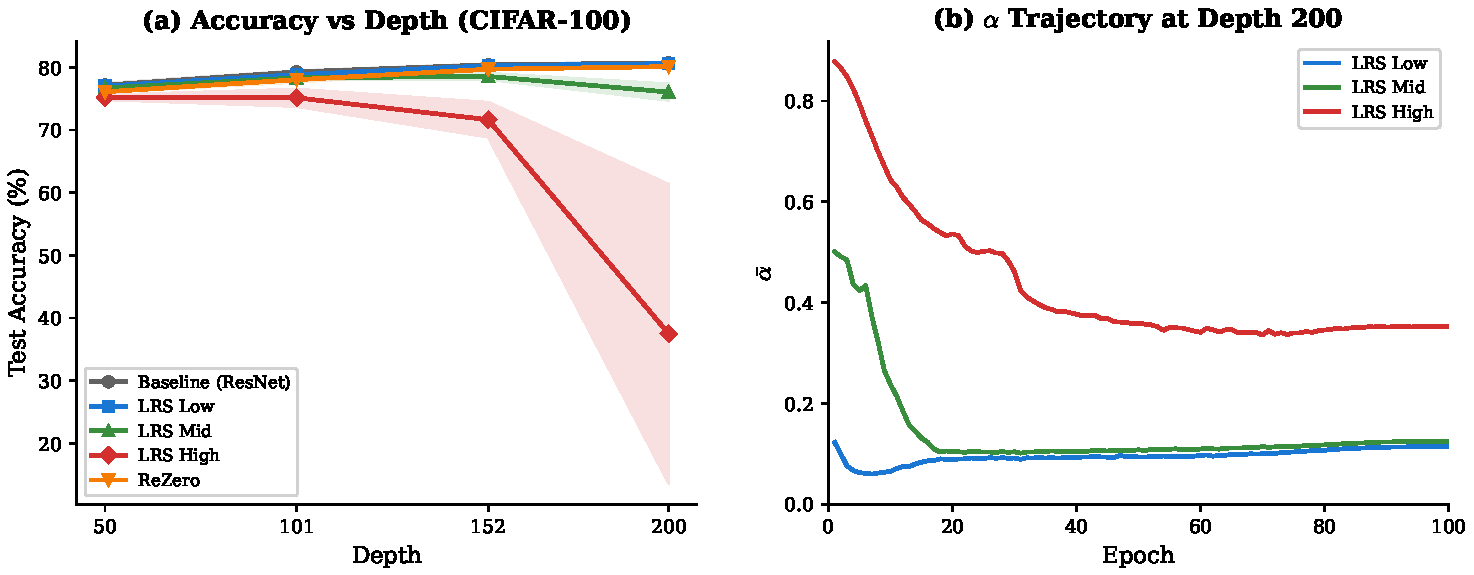
\includegraphics[width=0.85\linewidth]{figures/fig6_init_failure.pdf}
    \caption{CIFAR-100에서 세 가지 LRS 초기화에 따른 깊이별 정확도. LRS Low는 모든 깊이에서 안정적이며 baseline과 경쟁한다. LRS High는 점진적으로 저하되고 깊이 200에서 붕괴한다.}
    \label{fig:init_sensitivity}
\end{figure}

\subsection{고정 Alpha vs.\ 학습된 Alpha}
\label{sec:fixed_alpha}

$\alpha$를 \emph{학습}하는 것이 필수적인지---단순히 작은 고정 값을 사용하는 것이 아닌---검증하기 위해, CIFAR-100 깊이 152에서 학습된 LRS와 고정-$\alpha$ 변형을 비교한다.

\begin{table}[t]
\centering
\caption{깊이 152, CIFAR-100에서 고정 $\alpha$ vs.\ 학습된 $\alpha$. 학습된 평균에 가까운 고정 값이라도 블록별 학습의 성능에 미치지 못한다.}
\label{tab:fixed_alpha}
\begin{tabular}{lcc}
\toprule
\textbf{구성} & \textbf{정확도 (\%)} & \textbf{비고} \\
\midrule
학습된 (LRS Low) & \textbf{80.28} & 블록별 $\alpha$, 평균 $\approx 0.13$ \\
고정 $\alpha = 0.1$ & 79.81 & 학습된 평균에 근접 \\
고정 $\alpha = 0.3$ & 67.94 & 중간 수준 변환 \\
고정 $\alpha = 0.5$ & 44.19 & 표준 ResNet 비율 \\
고정 $\alpha = 0.7$ & 20.62 & 잔차 선호 \\
\midrule
Baseline ($\alpha = 0.5$ 암묵적) & 80.42 & 표준 ResNet (LRS 없음) \\
\bottomrule
\end{tabular}
\end{table}

결과는 인상적이다. 첫째, $\alpha = 0.5$ (표준 ResNet 비율, 보완적 항등 스케일링과 함께 균일하게 적용)는 44.19\%에 불과하여 baseline의 80.42\%보다 훨씬 낮다. 이는 고정-$\alpha$ 수식 $y = 0.5 F(x) + 0.5 x$가 양 분기를 명시적으로 반감시키기 때문이며, 전체 스케일을 보존하는 표준 ResNet의 $y = F(x) + x$와 다르다. 이는 LRS 수식이 $\alpha$가 학습되거나 작은 값으로 설정될 때만 의미 있음을 확인한다.

둘째, 학습된 평균 0.13에 가까운 고정 $\alpha = 0.1$조차 학습된 변형보다 0.47\% 낮은 성능을 보인다. 이 격차는 학습된 LRS가 다운샘플링 블록에 높은 $\alpha$ (0.42--0.96)를 할당하면서 일반 블록을 거의 0으로 유지하기 때문에 발생한다. 균일한 고정 값은 이 이질적 구조를 포착할 수 없다.

\begin{figure}[t]
    \centering
    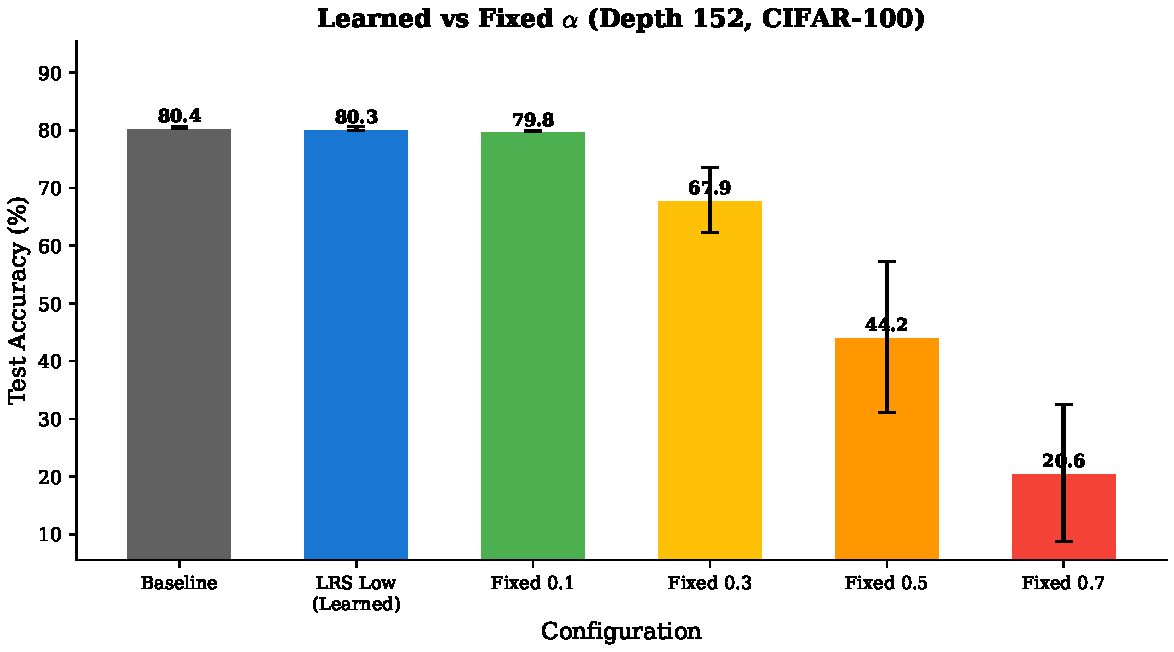
\includegraphics[width=0.85\linewidth]{figures/fig7_fixed_alpha.pdf}
    \caption{깊이 152, CIFAR-100에서의 고정 $\alpha$에 따른 정확도. 학습된 블록별 $\alpha$ (점선)가 모든 고정 값을 능가하여, 이질적 블록별 구조가 필수적임을 보여준다.}
    \label{fig:fixed_vs_learned}
\end{figure}

\subsection{항등 초기화 분석}
\label{sec:identity_init}

LRS에서 관찰된 낮은 유효 깊이가 표준 He 초기화의 부산물일 수 있다는 자연스러운 가설이 있다. He 초기화는 잔차 분기를 항등 보존 매핑이 아닌 무작위 가중치로 초기화한다. 잔차 분기가 항등 변환으로 시작한다면(``더 나은 출발점''을 제공), 네트워크가 더 많은 블록을 사용하도록 선택할까?

이를 검증하기 위해 표준 He 초기화와 부분적 및 전체 항등 초기화 방식을 비교한다. HybridA는 layer 3과 4(더 깊은 스테이지)를 항등 보존 가중치로 초기화하면서 layer 1과 2는 He 초기화를 유지한다. 모든 층에 대한 전체 항등 초기화도 검증한다. Table~\ref{tab:identity_init}은 CIFAR-100에서의 결과를 제시한다.

\begin{table}[t]
\centering
\caption{항등 초기화가 정확도와 학습된 $\alpha$에 미치는 영향 (CIFAR-100, 3-시드 평균 $\pm$ 표준편차). 전체 항등 초기화는 치명적으로 실패하는 반면, 부분 항등(HybridA) + LRS는 최고 정확도를 달성한다---그러나 유효 깊이는 변하지 않는다.}
\label{tab:identity_init}
\begin{tabular}{lcccc}
\toprule
\textbf{모델} & \textbf{d152 정확도 (\%)} & \textbf{d200 정확도 (\%)} & \textbf{$\alpha$ 평균 (d200)} & \textbf{활성 블록} \\
\midrule
Baseline (He 초기화) & 80.42$\pm$0.18 & 80.72$\pm$0.13 & --- & --- \\
LRS Low + He 초기화 & 80.28$\pm$0.31 & 80.65$\pm$0.01 & 0.114 & 5 / 66 \\
HybridA (Identity L3,4) & 80.02$\pm$0.26 & 80.40$\pm$0.17 & --- & --- \\
LRS Low + HybridA & \textbf{80.72$\pm$0.29} & \textbf{81.14$\pm$0.18} & 0.118 & 6 / 66 \\
ResNet (전체 Identity) & 13.41$\pm$0.41 & 12.98$\pm$0.16 & --- & --- \\
\bottomrule
\end{tabular}
\end{table}

이 실험에서 몇 가지 발견이 도출된다:

\textbf{전체 항등 초기화는 치명적으로 실패한다.} 모든 잔차 분기가 항등 변환으로 초기화되면, 네트워크는 거의 랜덤 수준의 성능(깊이 200에서 12.98\%)으로 붕괴한다. 무작위 초기화가 제공하는 다양성 없이는 네트워크가 대칭을 깨뜨리고 의미 있는 특징을 학습할 수 없다.

\textbf{부분 항등 초기화는 정확도를 향상시킨다.} HybridA(깊이 스테이지 3, 4에 대한 항등 초기화)와 LRS의 조합이 모든 구성에서 최고 정확도를 달성한다: 깊이 200에서 81.14\%로, 표준 baseline(80.72\%)과 표준 LRS Low(80.65\%) 모두를 능가한다.

\textbf{유효 깊이는 초기화에 불변이다.} 향상된 정확도에도 불구하고, 학습된 $\alpha$ 값은 표준 초기화와 항등 초기화 간에 거의 동일하다: 평균 $\alpha$ 0.114 vs.\ 0.118, 활성 블록 5개 vs.\ 6개(66개 중). 네트워크는 잔차 분기의 초기화 방식에 관계없이 동일한 유효 깊이로 수렴한다.

이 결과는 낮은 유효 깊이가 불량한 초기화의 부산물이라는 가설을 배제하기 때문에 중요하다. 잔차 분기가 항등 변환을 수행하도록 초기화되어---유용한 변환을 학습하기 위한 더 나은 출발점을 제공함---에도, 네트워크는 동일한 유효 깊이로 수렴한다. 이는 낮은 유효 깊이가 초기화에 의해 부과된 제한이 아닌 네트워크의 \emph{진정한 선호}를 반영함을 시사한다.

\subsection{블록 프루닝 검증}
\label{sec:pruning}

낮은 $\alpha$ 값을 가진 블록이 실제로 불필요한지 직접 검증하기 위해, 두 가지 프루닝 실험을 수행한다. 첫째, $\alpha$가 임계값 이하인 블록을 항등 사상으로 대체하고 재학습 없이 정확도를 측정한다. 둘째, 프루닝 후 10 에폭의 미세 조정(fine-tuning)을 적용하여 남은 블록이 적응할 수 있도록 한다. 각 bottleneck 블록은 6개의 layer(3개의 합성곱과 3개의 배치 정규화)로 구성된다.

\begin{table}[t]
\centering
\caption{CIFAR-100에서의 블록 프루닝 결과 (ResNet-200, 66 블록). ``No FT''는 블록 제거 후 즉시 평가; ``With FT''는 제거 후 10 에폭의 미세 조정 적용.}
\label{tab:pruning}
\begin{tabular}{lcccccc}
\toprule
\textbf{임계값} & \textbf{제거} & \textbf{Layer} & \textbf{남은} & \textbf{No FT} & \textbf{With FT} & $\mathbf{\Delta}$ \\
\midrule
없음 (원본) & 0 & 0 & 66 & 80.54\% & --- & --- \\
$\alpha < 0.03$ & 2 (3\%) & 12 & 64 & 80.54\% & --- & \textbf{0.00} \\
$\alpha < 0.05$ & 10 (15\%) & 60 & 56 & 73.88\% & 79.53\% & \textbf{$-$1.01} \\
$\alpha < 0.08$ & 37 (56\%) & 222 & 29 & 3.97\% & 76.22\% & $-$4.32 \\
$\alpha < 0.10$ & 48 (73\%) & 288 & 18 & 3.13\% & 74.83\% & $-$5.71 \\
$\alpha < 0.15$ & 58 (88\%) & 348 & 8 & 3.63\% & 72.64\% & $-$7.90 \\
\bottomrule
\end{tabular}
\end{table}

결과는 두 가지 중요한 발견을 보여준다. 첫째, $\alpha < 0.03$인 블록은 실제로 비활성 상태이다: 2개 블록(12개 layer)을 제거해도 \textbf{정확도 손실이 0\%}이며, $\alpha$가 불필요한 블록을 정확히 식별함을 확인한다.

둘째, 미세 조정이 회복을 극적으로 개선한다. 미세 조정 없이 15\%의 블록($\alpha < 0.05$)을 제거하면 정확도가 6.66\% 하락하지만, 단 10 에폭의 미세 조정으로 손실이 \textbf{1.01\%}로 감소한다. 56\%의 블록을 제거해도 76.22\% (80.54\%에서)로 회복되며, 73\% 제거 시에도 74.83\%를 달성한다. 이는 네트워크의 계산이 고도로 분산되어 있음을 보여준다: 개별 낮은 $\alpha$ 블록의 기여는 작지만, 미세 조정을 통해 남은 블록이 보상할 수 있으며, 이는 Veit 등~\cite{veit2016residual}의 앙상블 해석을 확인해준다.

\begin{figure}[t]
    \centering
    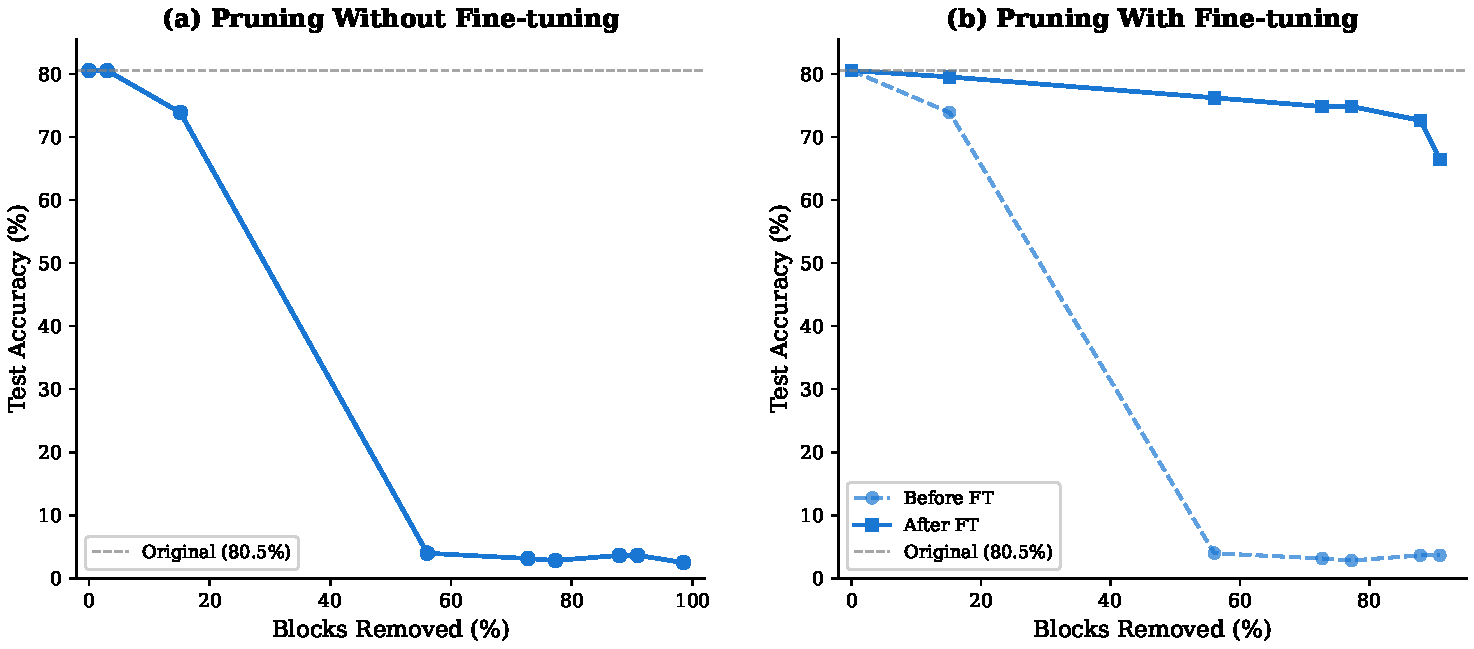
\includegraphics[width=\linewidth]{figures/fig11_pruning.pdf}
    \caption{CIFAR-100에서 ResNet-200의 블록 프루닝 결과. 왼쪽: 미세 조정 없이는 $\alpha < 0.03$ 블록만 안전하게 제거 가능. 오른쪽: 10 에폭의 미세 조정으로 15\%의 블록을 1\% 미만의 정확도 손실로 제거 가능하며, 56\% 제거 시에도 76\%로 회복.}
    \label{fig:pruning}
\end{figure}

\subsection{기존 방법과의 비교}
\label{sec:comparison_methods}

CIFAR-100 깊이 152에서 기존 잔차 스케일링 방법과 LRS를 비교하며, 모든 방법에 3개 시드를 사용한다(Table~\ref{tab:method_comparison}).

\begin{table}[t]
\centering
\caption{기존 잔차 스케일링 방법과의 비교 (깊이 152, CIFAR-100, 3-시드 평균). 모든 방법이 유사한 정확도를 달성하여, LRS의 가치가 성능 향상이 아닌 분석 능력에 있음을 확인한다.}
\label{tab:method_comparison}
\begin{tabular}{lc}
\toprule
\textbf{방법} & \textbf{정확도 (\%)} \\
\midrule
LayerScale & \textbf{80.56} \\
Baseline & 80.42 \\
LRS Low & 80.28 \\
Fixup & 79.79 \\
SkipInit / ReZero & 79.72 \\
\bottomrule
\end{tabular}
\end{table}

모든 방법이 0.84\%의 좁은 범위 내에서 수행되며, LayerScale이 약간 앞선다. 이 결과는 두 가지 이유에서 중요하다:

첫째, LRS가 분석 능력을 얻기 위해 성능을 희생하지 않음을 확인한다. LRS Low는 해석 가능한 블록별 $\alpha$ 값을 제공하면서 baseline과 0.14\% 이내의 정확도를 달성한다.

둘째, 방법들 간 성능의 유사성은 특정 스케일링 메커니즘보다 항등 선호 초기화 원칙이 더 중요하다는 관점을 뒷받침한다. ReZero ($\alpha = 0$에서 시작), SkipInit, LRS Low ($\alpha \approx 0.12$에서 시작) 모두 항등 근처에서 시작하여 비교 가능한 결과를 달성한다.

\begin{figure}[t]
    \centering
    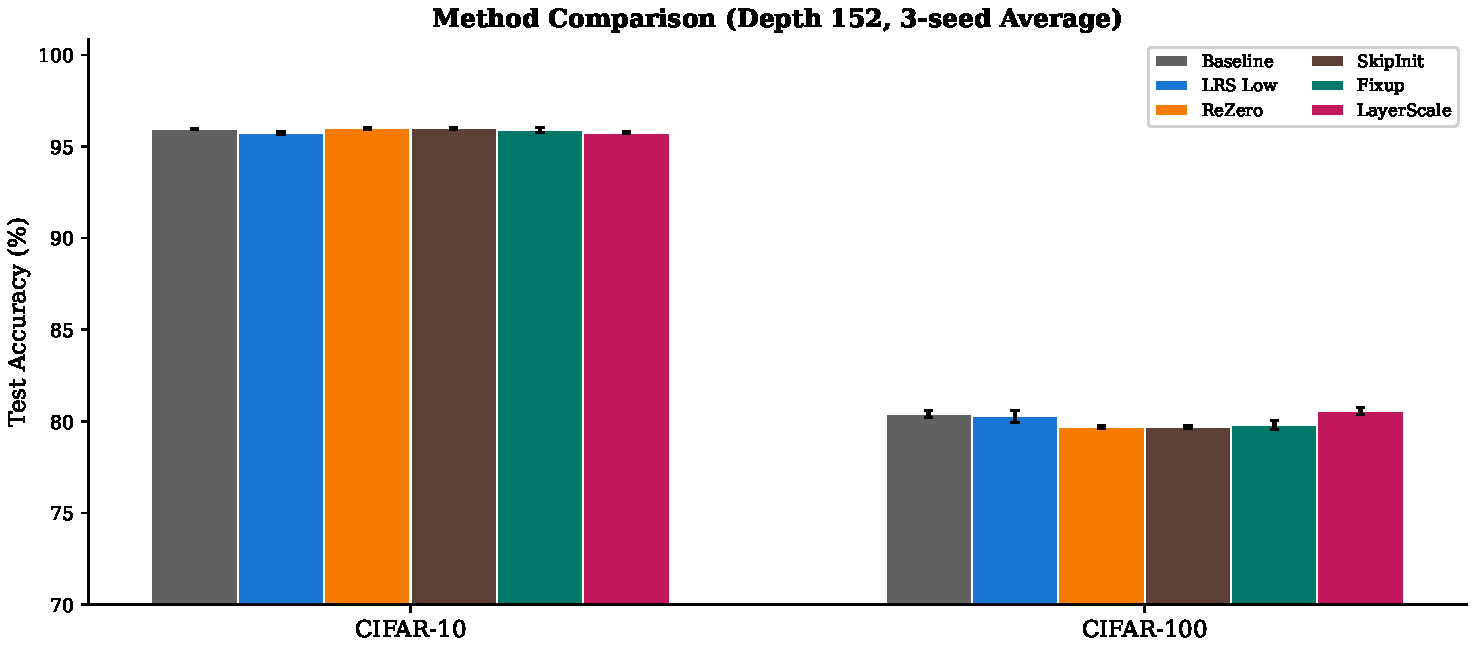
\includegraphics[width=0.85\linewidth]{figures/fig9_comparison.pdf}
    \caption{깊이 152, CIFAR-100에서의 잔차 스케일링 방법 정확도 비교. 모든 방법이 유사하게 수행되지만, LRS만이 $F(x)$와 $x$ 간의 해석 가능한 블록별 비율을 제공한다.}
    \label{fig:method_comparison}
\end{figure}

\subsection{ImageNet 검증}
\label{sec:imagenet}

발견의 대규모 검증을 위해 ImageNet에서 LRS 변형으로 ResNet-50을 학습한다(Table~\ref{tab:imagenet}).

\begin{table}[t]
\centering
\caption{ResNet-50을 사용한 ImageNet 검증 정확도. Top-1 및 Top-5 정확도를 보고한다.}
\label{tab:imagenet}
\begin{tabular}{lcc}
\toprule
\textbf{모델} & \textbf{Top-1 (\%)} & \textbf{Top-5 (\%)} \\
\midrule
Baseline & \textbf{75.86} & \textbf{92.92} \\
LRS High & 75.73 & 92.74 \\
LRS Mid & 75.62 & 92.73 \\
ReZero & 75.36 & 92.44 \\
LRS Low & 73.75 & 91.86 \\
LRS+HybridA Low & 72.32 & 91.02 \\
\bottomrule
\end{tabular}
\end{table}

ImageNet에서 baseline이 가장 높은 정확도를 달성하며, LRS 변형은 0.13--3.54\% 뒤처진다. 주목할 점은 LRS High가 ImageNet(depth 50)에서 75.73\%를 달성하여 baseline에 거의 근접한다는 것이다. 이는 CIFAR depth 200에서의 치명적 실패(37.50\%)와 극명하게 대조되며, 초기화 민감도가 높은 $\alpha$ 초기화의 본질적 결함이 아닌 깊이 의존적 현상임을 확인해준다. 특히 LRS Low의 이 성능 격차는 논의할 가치가 있다. 깊이 50 (16개 블록)에서 네트워크의 유효 깊이는 이미 명목 깊이에 가깝고 ($\alpha \approx 0.34$), LRS를 통한 블록 기여 감소가 이점을 제공하기 어려우며 네트워크의 용량을 제약할 수 있다. 더 깊은 깊이에서 LRS의 효과가 강한 것은 (CIFAR에서 ResNet-200으로 확인) LRS가 매우 깊은 네트워크에 대한 분석 및 학습 안정화 도구로서 가장 가치 있음을 시사한다.

ImageNet에서의 $\alpha$ 수렴 패턴은 CIFAR 발견과 일치한다: LRS Low는 동일 깊이의 CIFAR에서 관찰된 것과 유사한 평균 $\alpha$ 값으로 수렴하여, 깊이--$\alpha$ 관계의 데이터 독립성을 더욱 뒷받침한다.

\begin{figure}[t]
    \centering
    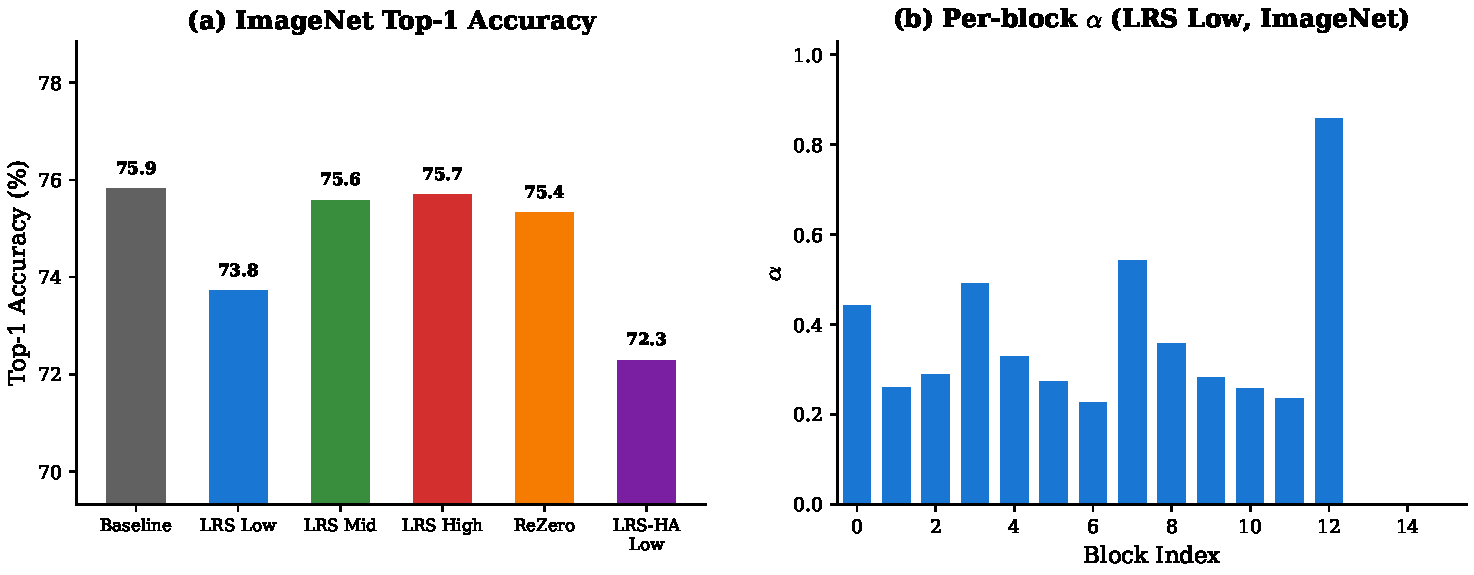
\includegraphics[width=0.85\linewidth]{figures/fig10_imagenet.pdf}
    \caption{ResNet-50을 사용한 ImageNet 검증 결과. Baseline이 정확도에서 앞서지만, 수렴된 $\alpha$ 패턴은 CIFAR 발견과 일치하여 깊이--$\alpha$ 관계의 일반성을 확인한다.}
    \label{fig:imagenet}
\end{figure}

%% ============================================================
\section{논의}
\label{sec:discussion}

\subsection{ResNet은 스스로 깊이를 선택한다}

본 연구의 핵심 발견은 심층 ResNet이 전체 깊이를 사용하지 않는다는 것이다. LRS로 학습된 200층 네트워크(66개 블록)는 변환을 5--6개 블록---주로 스테이지 경계---에 집중시키고, 나머지 60개 블록을 거의 항등 연산으로 축소한다. 네트워크는 명목 깊이의 약 8\%에 해당하는 유효 깊이를 자율적으로 선택했다.

전통적 관점에서 skip connection은 심층 네트워크의 기울기 흐름을 가능하게 함으로써 열화 문제를 ``해결''한다. 본 연구의 기울기 분석(Figure~\ref{fig:gradient_flow})은 skip connection이 실제로 기울기 흐름을 안정화함을 확인한다: skip connection이 없는 일반 네트워크는 초기 블록에서 $10^{13}$을 초과하는 기울기 폭발을 보이는 반면, ResNet은 66개 블록 전체에 걸쳐 관리 가능한 범위 내에서 기울기를 유지한다. 그러나 LRS는 네트워크가 이 안정성을 깊은 계산을 활용하기 위해서가 아니라 대부분의 블록을 \emph{우회}하기 위해 사용함을 드러낸다. LRS Low의 후반 블록에서의 거의 0에 가까운 기울기(Block~65에서 기울기 노름 $0.6$)는 $\alpha \approx 0$을 반영한다---네트워크는 이 블록들을 전혀 학습하지 않기로 선택한 것이다.

더 나아가, 항등 초기화 실험(Section~\ref{sec:identity_init})은 이 행동이 불량한 초기화의 부산물이 아님을 입증한다. 잔차 분기가 항등 변환으로 초기화되어---학습을 위한 이론적으로 더 나은 출발점을 제공함---에도, 네트워크는 동일한 유효 깊이(66개 중 5--6개 활성 블록, 평균 $\alpha \approx 0.11$--$0.12$)로 수렴한다. 초기화 방식에 걸친 이러한 불변성은 낮은 유효 깊이가 네트워크의 진정한 구조적 선호를 반영함을 강력하게 시사한다.

이러한 관찰은 열화 문제의 재해석으로 이어진다: 열화는 ``해결해야 할 문제''가 아니라 네트워크가 최적의 깊이를 선택하는 자연스러운 결과이다. Skip connection은 기울기 흐름을 방해하지 않으면서 블록이 거의 항등 연산으로 작동할 수 있게 함으로써 이 자기 선택의 \emph{메커니즘}을 제공한다. 네트워크는 깊이를 활용하지 못해서 열화하는 것이 아니다; 오히려, 불필요한 깊이를 사용하지 \emph{않을 수 있기 때문에} 성공하는 것이다.

이 발견은 잔차 네트워크의 ``반복적 추정 풀기(unrolled iterative estimation)'' 관점~\cite{greff2017highway}과 경로 앙상블 해석~\cite{veit2016residual}과 공명한다. 본 연구의 기여는 경로 분석이나 절제 연구로부터 간접적으로 추론하는 것이 아니라, 학습된 $\alpha$ 값을 통해 이 자기 선택을 \emph{직접 관측 가능}하게 만든 것이다.

\subsection{다운샘플링 블록의 역할}

블록별 분석은 모든 블록이 동등하지 않음을 드러낸다. 다운샘플링 블록(스테이지 경계에 위치)은 높은 $\alpha$ 값(0.42--0.96)을 유지하여, 공간 및 채널 차원 변경이 우회할 수 없는 필수적 변환임을 나타낸다. 이와 대조적으로, 스테이지 내의 많은 블록은 최소한으로 기여한다.

이는 설계 원칙을 제안한다: \textbf{스테이지의 수(따라서 다운샘플링 연산의 수)가 전체 블록 수보다 더 중요할 수 있다}. 각 2개 블록으로 구성된 4개 스테이지의 네트워크가 66개 블록 네트워크가 수행하는 유효 계산의 대부분을 포착할 수 있다.

\subsection{표준 ResNet은 왜 여전히 잘 작동하는가?}

자연스러운 질문은: 최적 $\alpha$가 0.5보다 훨씬 작다면, 표준 ResNet (LRS 관점에서 암묵적 $\alpha = 0.5$)은 왜 잘 작동하는가이다. 답은 중요한 구별에 있다. 표준 ResNet은 $y = F(x) + x$를 사용하며, $F(x)$와 $x$의 상대적 스케일을 제약하지 않는다. Batch normalization과 가중치 크기 조정을 통해 네트워크는 명시적 $\alpha$ 매개변수 없이도 효과적으로 작은 $\|F(x)\|/\|x\|$ 비율을 달성할 수 있다. LRS는 이 암묵적 비율을 명시적이고 관측 가능하게 만든다.

실제로, He et al.~\cite{he2016identity}과 De and Smith~\cite{de2020batch}는 batch normalization이 잔차 블록을 작은 $F(x)$ 쪽으로 편향시켜, 학습 가능한 스케일링 없이도 항등 선호의 한 형태를 효과적으로 구현함을 보였다. LRS는 이 현상을 확인하고 정량화한다.

\subsection{실용적 함의}

본 연구의 발견은 몇 가지 실용적 지침을 제안한다:

\begin{enumerate}
    \item \textbf{항등 선호 초기화가 필수적이다.} 어떤 형태의 잔차 스케일링을 사용하든, 항등 근처에서 시작하는 것($\alpha_0 \leq 0.12$)이 모든 깊이에서 안전하다. 잔차 선호 초기화는 피해야 한다.
    \item \textbf{깊이 효율성.} 블록의 ~8\%만 능동적으로 사용된다는 관찰은 추론 시 거의 항등인 블록을 가지치기하거나 단순화함으로써 상당한 모델 압축 잠재력이 있음을 시사한다.
    \item \textbf{아키텍처 탐색 가이드.} 이질적 $\alpha$ 분포(경계에서 높고 스테이지 내에서 낮음)는 신경망 아키텍처 탐색에 정보를 제공한다: 스테이지 내 블록을 추가하기보다 스테이지 전환에 용량을 할당하라.
\end{enumerate}

\subsection{제한사항}

본 연구에는 몇 가지 제한사항이 있다. 첫째, ImageNet 실험이 ResNet-50으로 제한되어 있으며, 더 깊은 ImageNet 모델(ResNet-101/152)이 대규모에서의 깊이--$\alpha$ 관계에 대한 더 강력한 검증을 제공할 것이다. 둘째, LRS는 블록당 하나의 매개변수를 추가하고 최적화 지형을 약간 수정하므로, 학습된 $\alpha$ 값은 표준 ResNet의 암묵적 선호가 아닌 이 수정된 지형을 반영한다. 셋째, 본 분석은 bottleneck ResNet에 한정되며 다른 아키텍처(예: LayerScale이 유사한 역할을 하는 Vision Transformer)에는 직접 적용되지 않을 수 있다. 넷째, 유효 깊이 임계값($\alpha > 0.3$)은 다소 임의적이며, 다른 임계값은 다른 유효 깊이 추정치를 산출할 것이지만, 대부분의 블록이 거의 항등이라는 정성적 결론은 견고하다.

%% ============================================================
\section{결론}
\label{sec:conclusion}

본 연구에서는 심층 잔차 네트워크가 블록 전체에 걸쳐 계산을 어떻게 분배하는지 관찰하기 위한 분석 도구로서 학습 가능한 잔차 스케일링(LRS)을 도입했다. 네 가지 깊이, 두 개의 CIFAR 데이터셋, ImageNet에 걸친 체계적 실험과 구성당 3개의 시드를 통해 다음을 입증했다:

\begin{enumerate}
    \item 심층 ResNet은 명목 깊이보다 훨씬 얕은 유효 깊이를 자율적으로 선택한다. 200층 네트워크에서 66개 블록 중 5--6개만이 의미 있는 변환을 유지하며, 나머지는 거의 항등 우회로 작동한다.
    \item 평균 학습된 $\alpha$는 깊이에 따라 체계적으로 감소하며 (깊이 50에서 $\alpha \approx 0.35$, 깊이 200에서 $\alpha \approx 0.11$), 이 패턴은 데이터셋에 크게 의존하지 않아 고유한 구조적 속성을 반영한다.
    \item 능동적 블록은 스테이지 경계(다운샘플링 연산)에 집중되어 있는 반면, 스테이지 내 블록은 점진적으로 항등으로 축소되어, 전체 깊이보다 스테이지 전환에서의 깊이가 더 중요함을 시사한다.
    \item 이 항등 선호를 존중하는 초기화가 극단적 깊이에서의 학습 성공의 필요조건이며, 이를 위반하면 치명적 붕괴가 발생한다.
    \item 기울기 분석은 skip connection이 기울기 흐름을 안정화하지만, 네트워크가 이 안정성을 대부분의 블록을 활용하기보다 우회하는 데 사용함을 보여준다. 후반 블록은 $\alpha \approx 0$을 반영하는 거의 0에 가까운 기울기를 보인다.
    \item 항등 초기화 실험은 낮은 유효 깊이가 초기화의 부산물이 아님을 확인한다: 항등 보존 잔차 분기에서도 네트워크는 동일한 유효 깊이(66개 중 5--6개 활성 블록)로 수렴하여, 이것이 진정한 구조적 선호임을 입증한다.
\end{enumerate}

이러한 발견은 잔차 네트워크 깊이에 대한 새로운 관점을 제공한다: ``네트워크를 얼마나 깊게 만들어야 하는가''를 묻는 대신, 관련된 질문은 ``과제가 얼마나 많은 스테이지 전환을 필요로 하는가''일 수 있다. 열화 문제는 해결해야 할 실패가 아니라 네트워크가 최적의 깊이를 선택하는 자연스러운 결과이다. Skip connection은 이 자기 선택의 메커니즘을 제공하며, LRS는 이를 가시적으로 만든다.

향후 연구에는 더 깊은 ImageNet 모델로의 LRS 분석 확장, 경량 대안으로서의 스테이지별 $\alpha$ 공유 탐구, 유효 깊이 개념의 모델 압축 적용, 그리고 Transformer 아키텍처에서 유사한 깊이 자기 선택이 발생하는지에 대한 조사가 포함된다.

%% ============================================================
\section*{CRediT 저자 기여 명세}
\textbf{주진호}: 개념화, 방법론, 소프트웨어, 검증, 형식적 분석, 조사, 원고 작성 -- 초안, 시각화.

\section*{이해충돌 선언}
저자는 이해충돌이 없음을 선언한다.

\section*{데이터 및 코드 가용성}
모든 코드, 학습된 모델, 실험 결과는 \url{https://github.com/Wlsghdh/Learnable_Residual_Scaling}에서 공개적으로 이용 가능하다.

%% ============================================================
\bibliographystyle{cas-model2-names}

\begin{thebibliography}{12}
\expandafter\ifx\csname natexlab\endcsname\relax\def\natexlab#1{#1}\fi
\providecommand{\url}[1]{\texttt{#1}}
\providecommand{\href}[2]{#2}
\providecommand{\path}[1]{#1}
\providecommand{\DOIprefix}{doi:}
\providecommand{\bibinfo}[2]{#2}

\bibitem[{He et~al.(2016a)}]{he2016deep}
\bibinfo{author}{K.~He}, \bibinfo{author}{X.~Zhang}, \bibinfo{author}{S.~Ren}, \bibinfo{author}{J.~Sun},
\bibinfo{year}{2016}a.
\bibinfo{title}{Deep residual learning for image recognition}.
\newblock In: \bibinfo{booktitle}{Proceedings of the IEEE Conference on Computer Vision and Pattern Recognition (CVPR)}, pp.~\bibinfo{pages}{770--778}.

\bibitem[{He et~al.(2016b)}]{he2016identity}
\bibinfo{author}{K.~He}, \bibinfo{author}{X.~Zhang}, \bibinfo{author}{S.~Ren}, \bibinfo{author}{J.~Sun},
\bibinfo{year}{2016}b.
\bibinfo{title}{Identity mappings in deep residual networks}.
\newblock In: \bibinfo{booktitle}{European Conference on Computer Vision (ECCV)}, pp.~\bibinfo{pages}{630--645}.

\bibitem[{Bachlechner et~al.(2021)}]{bachlechner2021rezero}
\bibinfo{author}{T.~Bachlechner}, \bibinfo{author}{B.P.~Majumder}, \bibinfo{author}{H.H.~Mao}, \bibinfo{author}{G.W.~Cottrell}, \bibinfo{author}{J.~McAuley},
\bibinfo{year}{2021}.
\bibinfo{title}{ReZero is all you need: Fast convergence at large depth}.
\newblock In: \bibinfo{booktitle}{Uncertainty in Artificial Intelligence (UAI)}, pp.~\bibinfo{pages}{1352--1361}.

\bibitem[{De and Smith(2020)}]{de2020batch}
\bibinfo{author}{S.~De}, \bibinfo{author}{S.L.~Smith},
\bibinfo{year}{2020}.
\bibinfo{title}{Batch normalization biases residual blocks towards the identity function in deep networks}.
\newblock In: \bibinfo{booktitle}{Advances in Neural Information Processing Systems (NeurIPS)}, vol.~\bibinfo{volume}{33}.

\bibitem[{Touvron et~al.(2021)}]{touvron2021going}
\bibinfo{author}{H.~Touvron}, \bibinfo{author}{M.~Cord}, \bibinfo{author}{A.~Sablayrolles}, \bibinfo{author}{G.~Synnaeve}, \bibinfo{author}{H.~J\'{e}gou},
\bibinfo{year}{2021}.
\bibinfo{title}{Going deeper with image transformers}.
\newblock In: \bibinfo{booktitle}{Proceedings of the IEEE/CVF International Conference on Computer Vision (ICCV)}, pp.~\bibinfo{pages}{32--42}.

\bibitem[{Zhang et~al.(2019)}]{zhang2019fixup}
\bibinfo{author}{H.~Zhang}, \bibinfo{author}{Y.N.~Dauphin}, \bibinfo{author}{T.~Ma},
\bibinfo{year}{2019}.
\bibinfo{title}{Fixup initialization: Residual learning without normalization}.
\newblock In: \bibinfo{booktitle}{International Conference on Learning Representations (ICLR)}.

\bibitem[{Veit et~al.(2016)}]{veit2016residual}
\bibinfo{author}{A.~Veit}, \bibinfo{author}{M.J.~Wilber}, \bibinfo{author}{S.~Belongie},
\bibinfo{year}{2016}.
\bibinfo{title}{Residual networks behave like ensembles of relatively shallow networks}.
\newblock In: \bibinfo{booktitle}{Advances in Neural Information Processing Systems (NeurIPS)}, vol.~\bibinfo{volume}{29}.

\bibitem[{Srivastava et~al.(2015)}]{srivastava2015highway}
\bibinfo{author}{R.K.~Srivastava}, \bibinfo{author}{K.~Greff}, \bibinfo{author}{J.~Schmidhuber},
\bibinfo{year}{2015}.
\bibinfo{title}{Highway networks}.
\newblock \href{http://arxiv.org/abs/1505.00387}{\tt arXiv:1505.00387}.

\bibitem[{Greff et~al.(2017)}]{greff2017highway}
\bibinfo{author}{K.~Greff}, \bibinfo{author}{R.K.~Srivastava}, \bibinfo{author}{J.~Schmidhuber},
\bibinfo{year}{2017}.
\bibinfo{title}{Highway and residual networks learn unrolled iterative estimation}.
\newblock In: \bibinfo{booktitle}{International Conference on Learning Representations (ICLR)}.

\bibitem[{Huang et~al.(2016)}]{huang2016deep}
\bibinfo{author}{G.~Huang}, \bibinfo{author}{Y.~Sun}, \bibinfo{author}{Z.~Liu}, \bibinfo{author}{D.~Sedra}, \bibinfo{author}{K.Q.~Weinberger},
\bibinfo{year}{2016}.
\bibinfo{title}{Deep networks with stochastic depth}.
\newblock In: \bibinfo{booktitle}{European Conference on Computer Vision (ECCV)}, pp.~\bibinfo{pages}{646--661}.

\bibitem[{Frankle and Carlin(2019)}]{frankle2019lottery}
\bibinfo{author}{J.~Frankle}, \bibinfo{author}{M.~Carlin},
\bibinfo{year}{2019}.
\bibinfo{title}{The lottery ticket hypothesis: Finding sparse, trainable neural networks}.
\newblock In: \bibinfo{booktitle}{International Conference on Learning Representations (ICLR)}.

\bibitem[{Huang et~al.(2017)}]{huang2017densely}
\bibinfo{author}{G.~Huang}, \bibinfo{author}{Z.~Liu}, \bibinfo{author}{L.~van~der~Maaten}, \bibinfo{author}{K.Q.~Weinberger},
\bibinfo{year}{2017}.
\bibinfo{title}{Densely connected convolutional networks}.
\newblock In: \bibinfo{booktitle}{Proceedings of the IEEE Conference on Computer Vision and Pattern Recognition (CVPR)}, pp.~\bibinfo{pages}{4700--4708}.

\end{thebibliography}

\end{document}
